\documentclass[10pt,a4paper,oneside]{book}

%Hello there. Don't know what to do?
	%Search for the %? or \fixme and fix/add stuff.
	%Check zapiski 2007, your notes and your memory and fix/add stuff
	%kul knjige imajo quote na začetku poglavij
%
%lol, windows newline bug poje to vrsto na začetku včasih :P
%\documentclass[10pt,a4paper,oneside]{book}

\usepackage[slovene]{babel}
\usepackage[utf8x]{inputenc}
\usepackage[fleqn]{amsmath}%fleqn - levo zamaknjene enačbe
\usepackage{amsfonts}
\usepackage{amssymb}
\usepackage{makeidx}
\usepackage{graphicx}
\usepackage[x11names, rgb]{xcolor}
\usepackage{tikz}
\usetikzlibrary{calc,automata,snakes,arrows,shapes,decorations,positioning,shapes.arrows,chains,shadows}

\usepackage{torstyle}
%?this feels too much like CSS hacks :(
%torstlye predloge:
%Definicija \Def{}
%Primer \Primer{}
%Prirejen itemize \begin{items}
\hypersetup{pdftitle={Teoretične osnove računalništva}}

\begin{document}
\begin{titlepage}
\begin{center}
%looks useful
%{\resizebox{15cm}{!}{Teoretične osnove računalništva}}\\[5pt]
\ \\[1cm]
{\Huge\bf Teoretične osnove računalništva}\\[1cm]
{\huge \today}\ \\[1.55cm]
%{\LARGE Zapiski predavanj 2010/2011}\\[15pt]%Odkar sem dodal kontekstno-odvisne in linearne, to ni več samo to :P
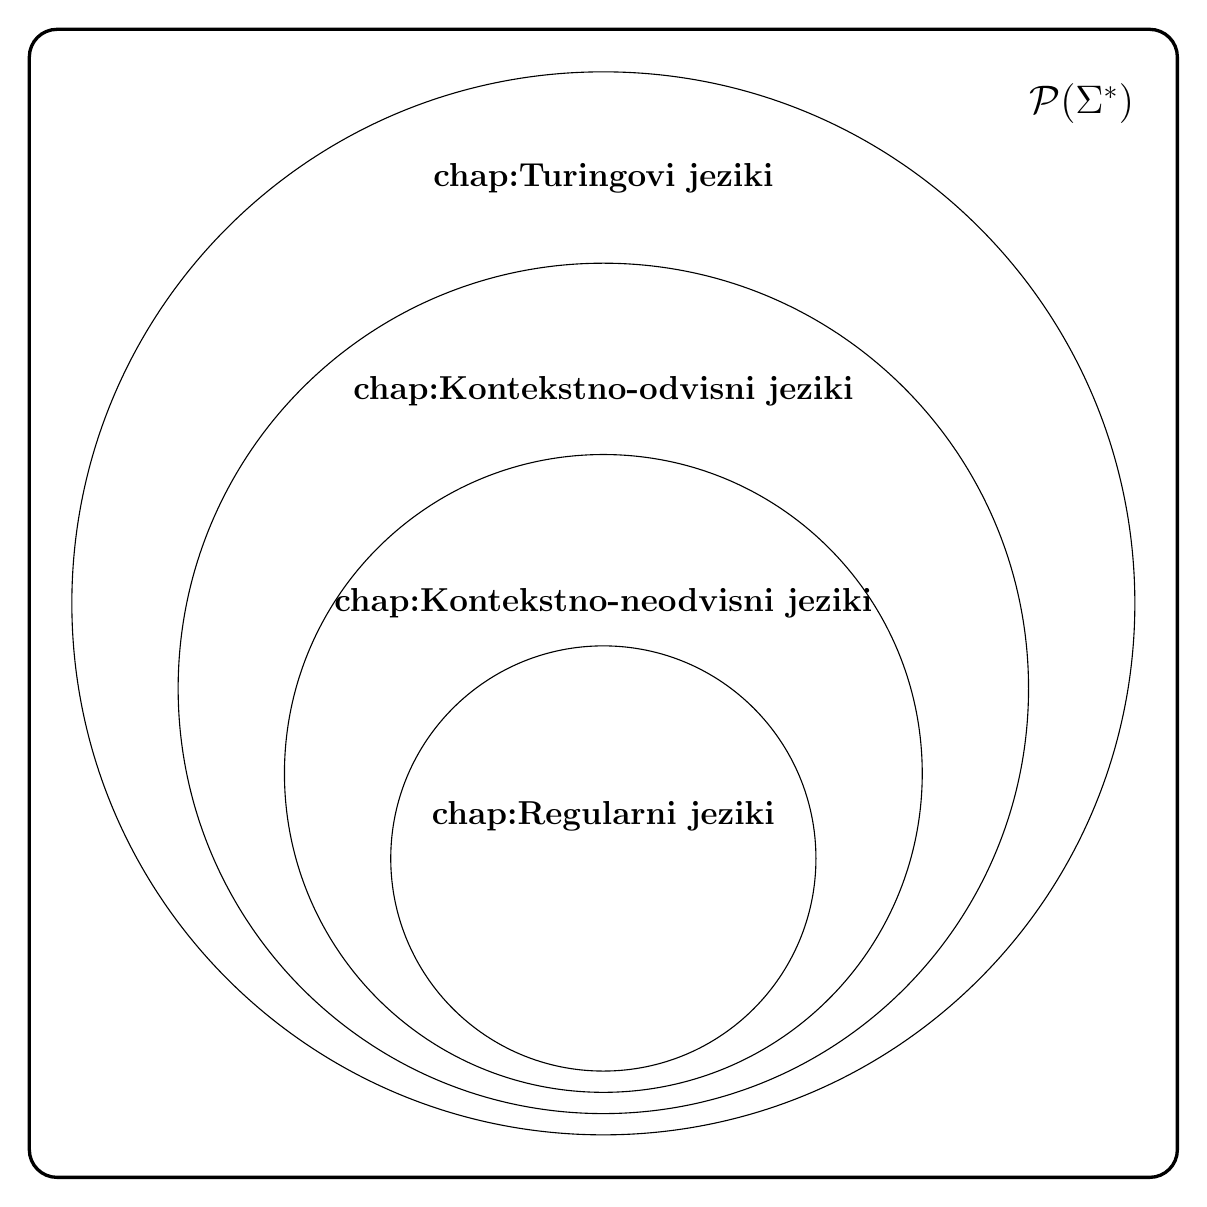
\begin{tikzpicture}[scale=1.35, very thick, circ/.style={thin}]%?tole ful upočasni pdflatex%, decorate, decoration={snake, amplitude=0.75pt}}]
	\draw [rounded corners=10pt] (-5.4cm,-5.4cm) rectangle (5.4cm,5.4cm);
	\node at (4.5cm,4.7cm) {\Large $\mathcal{P}(\Sigma^*)$};%sva šla vprašat... ker \Sigma^* znajo že RJ opisat, samo ne vseh možnih ;)

	\draw[circ] (0cm,0cm) circle (5cm);
	\node at (0,4cm) {\large\bf \nameref{chap:Turingovi jeziki}};

	\draw[circ] (0cm,-0.8cm) circle (4cm);
	\node at (0,2cm) {\large\bf \nameref{chap:Kontekstno-odvisni jeziki}};

	\draw[circ] (0cm,-1.6cm) circle (3cm);
	\node at (0,0cm) {\large\bf \nameref{chap:Kontekstno-neodvisni jeziki}};

	\draw[circ] (0cm,-2.4cm) circle (2cm);
	\node at (0,-2cm) {\large\bf \nameref{chap:Regularni jeziki}};
\end{tikzpicture}

\vfill
\parbox{7.5cm}{
\begin{center}

\includegraphics[width=0.15\textwidth]{./CC}\\[6pt]

This work is licensed under a Creative Commons Attribution-NonCommercial-ShareAlike 3.0 Unported License
\end{center}
}

\end{center}
\end{titlepage}
\tableofcontents
\pagebreak
%\newpage
%\sect{Notacija}
%\begin{itemize}
%	\item[Množice:] Označimo z velikimi tiskanimi črkami. Podamo jih lahko na naslednje načine\\
%	$ A = \{ a_1, a_1, a_3, \ldots \} $ - naštevanje elementov\\
%	$ B = \{ n | \ \mbox{pravilo za n} \} \ $ - opis elementov
%\end{itemize}

%?appendix this:
%\chapter{Slovar}
%?zihr obstaja neki za to, sicer naredi definitions okolje
%\begin{items}
%\item Razred - razred je množica elementov, ki ga lahko podamo z naštevanjem elementov ali z opisom lastnosti (opisni ali konceptualni razredi)
%\end{items}

\pagebreak
\chap{Uvod}
\sect{Matematične osnove}
\subsect{Teorija množic}
\subsect{Dokazovanje}
\subsubsection{Dokaz s konstrukcijo}
Dokaz obstoja nekega matematičnega objekta je to, da nam ga uspe sestaviti.

\begin{primeri}
\item Za vsak $n>4$, obstaja dvojiško drevo, ki ima natanko $3$ liste.\\
	Primer za $n=5$:
	\br
	\hspace*{1cm}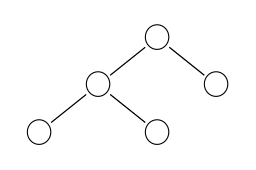
\begin{tikzpicture}[level distance=6mm, inner sep=-0.3mm]
		\node (root) {$\bigcirc$}
		child { node (a) {$\bigcirc$} 
			child { node (b) {$\bigcirc$} }
			child { node (c) {$\bigcirc$} }
		}
		child { node (d) {$\bigcirc$} };
	\end{tikzpicture}
	\br
	Primer za $n>5$, pri čemer je "$...$", poljubno vejitev samo v levo:
	\br
	\hspace*{1cm}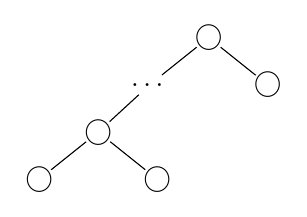
\begin{tikzpicture}[level distance=6mm, inner sep=-0.3mm]
		\node (root) {$\bigcirc$}
		child { node (a) [inner sep=1mm] {$\dots$} {
			child { node (b) [left=0.5cm] {$\bigcirc$} 
				child { node (c) {$\bigcirc$} }
				child { node (d) {$\bigcirc$} }}
		}}
		child { node (e) {$\bigcirc$} };
	\end{tikzpicture}
	\\
\item $| \mathbb{R} | = | [0,1) |$.\\
	\begin{items}
	\item Množici imata enako moč, kadar med njima obstaja bijektivna preslikava.
	\item Vsako realno število $r$ lahko zapišemo kot:
	\[ r=\pm d_1 d_2 \cdots d_n . \overline{d_1}\overline{d_2} \cdots \overline{d_m} \cdots;\ d_1 \neq 0 \]
	\item Definiramo preslikavo:
	\[ \mathbb{R}\rightarrow [0,1): r \rightarrow 0.s\overline{d_1} d_{n} \overline{d_2} d_{n-1} \cdots \overline{d_{n-1}} d_2 \overline{d_n} d_1 \overline{d_{n+1}} 0\overline{d_{n+2}} 0 \cdots \]
	kjer $s$ določa predznak ($s=0$, če $r \ge 0$ in $s=1$, sicer).
	\item Vidimo:
		\begin{items}
		\item $|\mathbb{R}|\ge |[0,1)|$, ker velja $[0,1) \subset \mathbb{R}$
		\item $|\mathbb{R}|\le |[0,1)|$,\fixme%?(ker se $0.2$ ne da preslikati v $\mathbb{R}$)??
		\end{items}
	\item Iz tega lahko sklepamo, da velja $|\mathbb{R}|=|[0,1)|$
	\end{items}
\end{primeri}
	
\subsubsection{Dokaz z indukcijo}
Če je množica induktivni razred%\footnote{Glej slovarček na koncu.}
, lahko z matematično indukcijo dokazujemo neko lastnost članov množice. Induktivni razred $I$ sestavlja:
\begin{items}
\item Baza indukcije - najbolj osnovna množica elementov (osnovni razred)
\item Pravila generiranja - kako iz elementov baze gradimo nove elemente (množico)
\end{items}
\begin{primeri}
\item Induktivni razred naravnih števil $(\mathbb{N})$
	\begin{items}
	\item Baza: $1 \in \mathbb{N}$ 
	\item Pravila generiranja: $n \in \mathbb{N} \Longrightarrow n+1 \in \mathbb{N} $
	\end{items}
\item Hilbertove krivulje \fixme
\end{primeri}

\subsubsection{Dokaz s protislovjem}
Vzamemo nasprotno trditev, od tiste, ki jo želimo preveriti in pokažemo, da to vodi v protislovje.

\begin{primeri}
\item Praštevil je končno mnogo.
	\begin{items}
	\item Predpostavimo, da poznamo vsa praštevila:\\
		$P = \{2,3,5,...,p\}$, kjer je $p$ zadnje praštevilo 
	\item Po definiciji obstajajo le praštevila in sestavljena števila (to so taka, ki jih lahko razstavimo na prafaktorje). 
	\item Če pomnožimo vsa znana praštevila iz $P$ in prištejemo $1$ dobimo število, ki se ga ne da razstaviti na prafaktorje iz množice $P$:\\
		$q = 2 * 3 * 5 * ... * p + 1$
	\item Torej je $q$ ali praštevilo (ker ni sestavljeno), ali pa število, sestavljeno iz prafaktorjev, ki jih ni v množici $P$.
	\item Oboje kaže na to, da v množici $P$ nimamo vseh praštevil, ter, da to velja za vsako končno množico praštevil.
	\end{items}
\item $\sqrt[3]{2}$ je racionalno število.
	\begin{items}
	\item Če je $\sqrt[3]{2}$ racionalno število, ga je moč zapisati kot ulomek $\frac{a}{b}$.
	\item Predpostavimo, da je ulomek $\frac{a}{b}$ okrajšan (torej, da velja: $GCD(a,b)=1$):
		\begin{align*}
		\sqrt[3]{2} &= \frac{a}{b}\\
		2 &= \left( \frac{a}{b} \right)^3\\
		2b^3 &= a^3
		\end{align*}
	\item Opazimo, da je $a$ sodo število, torej lahko pišemo $a = 2k$:
		\begin{align*}
		2b &= \left( 2k\right)^3\\
		2b &= 8k\\
		b &= 4k
		\end{align*}
	\item Ker se je pokazalo, da je tudi $b$ sodo število, $GCD(a,b)=1$ ne more držati, torej smo prišli v protislovje in s tem dokazali, da $\sqrt[3]{2}$ ni racionalno število.
	\end{items}
\end{primeri}
\sect{Osnove teorije jezikov}
\subsect{Uporabljene oznake}
\begin{items}
\item $a$ - znak ali simbol (niz dolžine 1)
\item $\Sigma$ - abeceda (končna neprazna množica znakov)
\item $w$ - niz ali beseda (poljubno končno zaporedje znakov $w_1w_2 \ldots w_n$)
\item $|w|$ - dolžina niza
\item $\varepsilon$ - prazen niz, $|w|=0$
\item $\Sigma^*$ - vsi možni nizi abecede
\end{items}

\subsect{Operacije nad jeziki}
\subsubsect{Stik nizov}
	\begin{align*}
	w  &= a_1 a_2 \dots a_n\\
	x  &= b_1 b_2 \dots b_m\\
	wx &= a_1 a_2 \dots a_n b_1 b_2 \dots b_m
	\end{align*}
\subsubsect{Stik}
	\begin{align*} 
	A & = \{ w_1 ,\ w_2 ,\ \dots ,\ w_n \} \\ 
	B & = \{ x_1 ,\ x_2 ,\ \dots ,\ x_m \} \\ 
	A \cdot B & = \{ w_ix_j \ | \ w_i \in A \ \wedge \ x_i \in B \}
	\end{align*} 
\subsubsect{Potenciranje}
	\begin{align*} 
	A^0 & = \{ \varepsilon \} \\
	A^k & = A \cdot A \cdot \ldots \cdot A \ = \ \bigcirc_{i=1}^{k} A \\
	\end{align*}
\subsubsect{Iteracija}
	\begin{align*} 
	A^* &= A^0 \cup A^1 \cup A^2 \cdots  \ = \ \bigcup_{i=0}^{ \infty } A^i
	\end{align*} 		
\subsubsect{Obrat}
	\begin{align*}
	w  &= a_1 a_2 \dots a_{n-1} a_n\\
	w^R  &= a_n a_{n-1} \dots a_2 a_1\\
	\end{align*}

\chap{Regularni jeziki}
\sect{Regularni izrazi}\label{sec:RI}
\Def{Imamo tri osnovne izraze:
	\begin{items}
	\item $\underline{\emptyset}$ je opisuje prazen jezik $ L(\underline{\emptyset})= \{ \}$
	\item $\underline{ \varepsilon }$ opisuje jezik $L(\underline{ \varepsilon })= \{ \varepsilon\}$
	\item $\underline{a}$ opisuje jezik $L( \underline{a} ) = \{ a \},\ a \in \Sigma$
	\end{items}
	In tri pravila za generiranje sestavljenih izrazov:
	\begin{items}
	\item $(r_1 + r_2)$ opisuje unijo jezikov $L(r_1 + r_2) = L(r_1) \bigcup L( r_2)$
	\item $(r_1\ r_2)$ opisuje stik jezikov $L(r_1\ r_2) = L(r_1)\cdot L( r_2)$
	\item $(r^*)$ opisuje iteracijo jezika $(L(r))^*$
	\end{items}
}
\begin{primeri}
\item Opiši vse nize, ki se končajo z nizom $00$ v abecedi $\Sigma = \{ 0,1 \}$.
	\[ r = (0+1)^*00 \]
	\item Opiši vse nize, pri katerih so vsi $a$-ji pred $b$-ji in vsi $b$-ji pred $c$-ji v abecedi $\Sigma = \{ a,b,c \}$.
		\[ a^*b^*c^* \]
	\item Opiši vse nize, ki vsebujejo vsaj dva niza '$aa$', ki se ne prekrivata v abecedi $\Sigma = \{ a,b,c \}$.
		\[ (a+b+c)^* aa (a+b+c)^* aa (a+b+c)^* \]
	\item Opiši vse nize, ki vsebuje vsaj dva niza '$aa$' ki se lahko prekrivata v abecedi $\Sigma = \{ a,b,c \}$
		\[ (a+b+c)^* aa (a+b+c)^* aa (a+b+c)^* + (a+b+c)^* aaa (a+b+c)^* \]
	\item Opiši vse nize, ki ne vsebujejo niza $11$ v abecedi $\Sigma = \{ 0,1 \}$
		\[ (\varepsilon  + 1 )(0^*01)^* 0^*	\]
		\[ (\varepsilon  + 1 )(0^* + 01)^* \]
	\item S slovensko abecedo opiši besedo "Ljubljana" v vseh sklonih in vseh mešanicah velikih in malih črk.
		\[ (L+l)(J+j)(U+u)(B+b)(L+l)(J+j)(A+a)(N+n)( (A+a)(O+o)(E+e)(I+i) ) \]
		Koliko različnih nizov opišemo s tem regularnim izrazom?\\
		\[ 2^8 \cdot 2^3 = 2^{11} \mbox{ nizov} \]
\end{primeri}
\sect{Končni avtomati}\label{sec:KA}
\subsect{Nedeterministični končni avtomati z $\varepsilon$-prehodi }
\Def{$\varepsilon$NKA je definiran kot peterka $M = \langle Q, \Sigma, \delta ,q_0 , F \rangle$, kjer je:
	\begin{items}
	\item $ Q $ - končna množica stanj
	\item $ \Sigma $ - vhodna abeceda
	\item $ \delta $ - funkcija prehodov, $\delta : Q \times (\Sigma \cup \{\varepsilon\}) \rightarrow 2^Q$
	\item $ q_0 $ - začetno stanje
	\item $ F $ - množica končnih stanj
	\end{items}
}
%?razlaga potenčne množice bi šla lahko nekam med mat. osnove... imam še en kup stvari o teoriji množic nekje. Drugač je pa kul - epsilon-closure je že napol opisan :)
$2^Q=P(Q)$ je tu potenčna množica stanj avtomata. To pomeni da je so v $2^Q$ vse možne kombinacije stanj. Recimo da se nahajamo v stanju A, potem nas funkcija prehodov $ \delta $ pripelje v vsa mozna stanja do katerih pridemo iz $A$ z določenim znakom abecede in z vsemi $ \varepsilon $ prehodi, naprimer $ \{ A_1,A2, \ldots , A_n \}$. Tukaj je množica stanj $ \{ A_1,A2, \ldots , A_n \} $ element potenčne množice $P(Q)$

\subsect{Nedeterministični končni avtomati}
\Def{NKA je definiran kot peterka $M = \langle Q, \Sigma, \delta, q_0, F \rangle$, kjer je:
	\begin{items}
	\item $ Q $ - končna množica stanj
	\item $ \Sigma $ - vhodna abeceda
	\item $ \delta $ - funkcija prehodov $\delta : Q \times \Sigma \rightarrow 2^{Q}$
	\item $ q_0 $ - začetno stanje
	\item $ F $ - množica končnih stanj
	\end{items}		
}
\Def{Funkcija $\varepsilon$-closure($q$) nam pove, do katerih stanj lahko pridemo iz stanja $q$ po $\varepsilon$ prehodih.
	\[ \varepsilon\mbox{-closure}(q) = \{ q_k\ |\ \exists q_1, q_2, \dots q_n \in Q,\ q=q_1 \wedge q_i \in \delta(q_{i-1}, \varepsilon) \} \]
}
\Def{Posplošena funkcija prehodov $\hat\delta$ nam pove, do katerih stanj pridemo po nekem nizu.		\[ \hat\delta(q, \varepsilon) = \varepsilon\mbox{-closure}(q) \]
	\[ \hat\delta(q, a) = \delta(q, a) \]
	\[ \hat\delta(q, wa) = \varepsilon\mbox{-closure}(\{ q''\ |\ q' \in \hat\delta(q, w) \wedge q'' \in \delta(q', a) \})\]
}

\subsect{Deterministični končni avtomat}
\Def{DKA je definiran kot petorka $M = \langle Q, \Sigma, \delta, q_0, F \rangle$, kjer je:
	\begin{items}
	\item $ Q $ - končna množica stanj
	\item $ \Sigma $ - vhodna abeceda
	\item $ \delta $ - funkcija prehodov, $\delta : Q \times \Sigma \rightarrow Q$
	\item $ q_0 $ - začetno stanje
	\item $ F $ - množica končnih stanj
	\end{items}	
}

\subsect{Jeziki končnih avtomatov}
\Def{Jezik $\varepsilon$NKA ter NKA je definiran kot:
	\begin{equation*}
	L=\{ w\ |\ \hat\delta(q_0, w) \cap F \neq \emptyset \}
	\end{equation*}
	kjer je $\hat\delta(q,w)$ posplošena funkcija prehodov v večih korakih.}
\Def{Jezik DKA je definiran kot:
	\begin{equation*}
	L=\{ w\ |\ \hat\delta(q_0, w) \in F \}
	\end{equation*}
}
Definicije želijo povedati, da so v jeziku točno tisti nizi, po katerih je iz začetnega stanja mogoče priti do nekega končnega stanja.

\sect{Levo in desno-linearne gramatike}\label{sec:LLGDLG}
Posebnost linearnih gramatik je v tem, da imajo na desni strani produkcij največ en vmesni simbol, ampak ta model je že nekoliko močnejši od regularnih jezikov (glej \ref{sec:LG}), če pa se omejimo le na tiste produkcije, ki imajo ta edini vmesni simbol vedno na skrajno levi strani, ali pa vedno na skrajni desni strani niza, dobimo model, ki opisuje regularne jezike.
%
\Def{Linearna gramatika je definirana kot četvorček $G=\langle N,T,P,S \rangle$, kjer je:
\begin{items}
\item N - množica spremenljivk oz. vmesnih simbolov, $N \subseteq \Sigma$
\item T - množica znakov oz. končnih simbolov, $T \subset \Sigma,\ N\cap T = \emptyset$
\item P - množica produkcij
\item S - začetni simbol, $S \in N$
\end{items}
Pri tem je abeceda $\Sigma = N \cup T$ in $N\cap T = \emptyset$.
}
\subsect{Produkcije}
\Def{Pri levo in desno-linearnih gramatikah, s produkcijami slikamo nek vmesni simbol v niz, ki ima lahko vmesni simbol le na skrajno levi pri levo-linearnih, oz. le na skrajno desni pri desno-linearnih:
	\begin{items}
	\item $P \subset N \times ((N\cup \{\varepsilon\})T^*)$ - pri levo-linearnih gramatikah
	\item $P \subset N \times (T^* (N\cup \{\varepsilon\}))$ - pri desno-linearnih gramatikah
	\end{items}
	%neko moje bluzenje... mogoče je prov.
	%\[ \left[ A \rightarrow B \beta \right] \in P \mbox{ pri levo, ter}\]
	%\[ \left[ A \rightarrow \beta B \right] \in P \mbox{ pri desno-linearnih gramatikah}\]
	%\[ A \in V,\ \ B \in (V \cup \{\varepsilon\}),\ \ \beta \in T^* \]
}
\subsect{Relacija izpeljave $\Rightarrow$}
\Def{Relacija izpeljave pri levo in desno-linearnih gramatikah prek neke produkcije iz $P$, slika trenutni niz v nov niz, tako, da ima novi niz vmesne simbole lahko le na skrajni levi, pri desno-regularnih pa le na skrajno desni strani, torej:
	\begin{items}
	\item $\left[ A \rightarrow B \beta \right]$ - pri levo-linearnih gramatikah
	\item $\left[ A \rightarrow \beta B \right]$ - pri desno-linearnih gramatikah
	\end{items}
	Pri tem je $A \in N,\ B \in (N \cup \{\varepsilon\}),\ \beta \in T^*$
}
\Def{Kadar želimo pokazati, da je mogoče z enim ali več koraki mogoče priti iz enega niza do drugega, to lahko zapišemo s posplošeno relacijo izpeljave $\Rightarrow^*$.
	%homebrew definicija
	\[ \alpha \Rightarrow^* \beta \mbox{\ \ \ n.t.k.\ \ \ } \alpha = \alpha_0 \Rightarrow \alpha_1 \Rightarrow \dots \Rightarrow \alpha_k = \beta;\ k>0 \]
}
\subsect{Jezik gramatik}

\sect{Jezik regularnih jezikov}
%?tu bi pasal dokazi :)
\Def{Jezik ki ga opisuje poljubni regularni izraz, končni avtomat, levo ali desno-linearna gramatika, je regularni jezik.}
Regularni jeziki ne vsebujejo informacije o prejšnjih znakih vhodnega niza in se z njimi ne da opisati poljubnega jezika. (za postopke dokazovanja regularnosti glej \ref{sec:Dokazovanje RJ}).
\begin{primeri}
	%\item $\Sigma^* $ je regularni izraz %?wrong... jezik je nujno strogi subset \sigma*... ker ni dovolj močnega modela za opis vseh možnih nizov
	\item $L =\{ \}$ - prazen jezik
	\item $L = \{ \varepsilon \}$ - jezik, ki vsebuje $\varepsilon$ (ni prazen)
	\item $L = \{ a, aa, ab \}$ - jezik, ki vsebuje nize "a, aa, ab"
	\item $L = \{ 0^n 1^n \ | \ n > 0 \} $ - jezik, ki \underline{ni} regularen (ne moremo si zapomniti poljubnega števila $n$)
\end{primeri}

\sect{Ohranjanje regularnosti jezikov}
Regularnost jezika že po definiciji ohranjajo operacije:
\begin{items}
\item $L_1 \cup L_2$ - unija 
\item $L_1 \cdot L_2$ - stik 
\item $L^*$ - iteracija
\end{items}
Obstajajo postopki za konstrukcijo, ki kažejo, da regularnost ohranjajo tudi:
\begin{items}
\item $L_1 \cap L_2$ - presek\\
	Iz avtomatov za $L_1$ in $L_2$ zgradimo t.i. produktni avtomat:
		\begin{align*}
			M_{L_1} &= \{ Q_1, \Sigma, \delta_1, q_{1_0}, F_1 \}\\
			M_{L_2} &= \{ Q_2, \Sigma, \delta_2, q_{2_0}, F_2 \}\\
			M_{L_1}*M_{L_2} &= \{ Q_1 \times Q_2, \Sigma, \delta_*, \langle q_{1_0}, q_{2_0} \rangle, F_1 \times F_2 \}
		\end{align*}
	Namesto stanj dobimo pare stanj in moramo preveriti v kateri par pridemo, če gledamo oba stara avtomata, končna pa so tista stanja, ki so končna v obeh starih avtomatih.
	\[ \delta_*(\langle q_1, q_2 \rangle, a) = \langle \delta_1(q_1, a), \delta_2(q_2, a)\rangle \]
\item $L^R$ - obrat\\
	Obrnemo vse povezave, ustvarimo novo začetno stanje, ki gre po $\varepsilon$ v stara končna, staro začetno stanje pa postane edino končno stanje.
\end{items}
Regularnost ohranjajo tudi vse operacije, ki so sestavljene iz zgoraj naštetih:
\begin{items}
\item $L_1 \setminus L_2 = L_1 \cap \overline L_2$ - razlika
\item $\overline{L} = \Sigma^* \setminus L$ - komplement
\item $L_1 \underline\vee L_2 = (L_1 \cup L_2) \setminus (L_1 \cap L_2)$ - ekskluzivni ali 
\end{items}

\sect{Prevedbe med modeli regularnih jezikov}
Regularni izrazi, regularne gramatike in končni avtomati so enako močni modeli in je mogoče pretvarjati med njimi. V tem odseku bomo predstavili naslednje prevedbe:\\[12pt]%?ustrezno dopolni :)
\begin{center}
\begin{tikzpicture}[>=latex',/tikz/initial text=""]
	\node (RI)   at (0bp,0bp)   {RI};
	\node (eNKA) at (75bp,0bp)  {$\varepsilon$NKA};
	\node (NKA)  at (150bp,0bp) {NKA};
	\node (DKA)  at (225bp,0bp) {DKA};
	\node (DLG)  at (300bp,0bp) {DLG};
	\node (LLG)  at (375bp,0bp) {LLG};

	\draw [bend left,->]  (DKA) to node[auto] {\ref{KA-RI}} (RI);
	\draw [bend right,->]  (DLG) to node[auto] {\ref{DLG-eNKA}} (eNKA);
	\draw [->]  (DKA) to node[auto] {} (NKA);
	\draw [->]  (NKA) to node[auto] {} (eNKA);
	\draw [->]  (RI) to node[auto] {\ref{RI-eNKA}} (eNKA);
\end{tikzpicture}
\end{center}

	%nekako tako mam v lanskih vajah, vrjetno mam letos bl prov :)
	%ps. lanske vaje so ful ugly, tko d si nism kj velik pomagov
	%\subsubsection{KA $\rightarrow$ DLG}
	%\subsubsection{DLG $\rightarrow$ KA}
	%\subsubsection{KA $\rightarrow$ RI}
	%\subsubsection{NKA $\rightarrow$ DKA}
	%\subsubsection{$\varepsilon$-NKA $\rightarrow$ NKA}
	%\subsubsection{RI $\rightarrow$ $\varepsilon$-NKA}
\subsect{Regularni izraz $\rightarrow$ Nedeterministični končni avtomat z $\varepsilon$-prehodi}\label{RI-eNKA}
%konstanta
\def\RIeNKAscale{0.60}

Pretvoriti moramo le osnovne in sestavljene regularne izraze, nato pa ustrezne avotmate samo povezujemo skupaj.
\begin{center}
\begin{minipage}[t]{6cm}
Osnovni izrazi:
\begin{itemize}
\item $r = \emptyset$\\
\begin{tikzpicture}[>=latex',/tikz/initial text="", scale=\RIeNKAscale, every state/.style={scale=\RIeNKAscale}]]
	\node (q0) at (0bp,0bp)  [state, initial]   {};
	\node (q1) at (80bp,0bp) [state, accepting] {};
\end{tikzpicture}
\item $r = \varepsilon$\\
\begin{tikzpicture}[>=latex',/tikz/initial text="", scale=\RIeNKAscale, every state/.style={scale=\RIeNKAscale}]]
	\node (q0) at (0bp,0bp)  [state, initial]   {};
	\node (q1) at (80bp,0bp) [state, accepting] {};

	\draw [->] (q0) to node[auto] {$\varepsilon$} (q1);
\end{tikzpicture}
\item $r = a$\\
\begin{tikzpicture}[>=latex',/tikz/initial text="", scale=\RIeNKAscale, every state/.style={scale=\RIeNKAscale}]]
	\node (q0) at (0bp,0bp)  [state, initial]   {};
	\node (q1) at (80bp,0bp) [state, accepting] {};

	\draw [->] (q0) to node[auto] {$a$} (q1);
\end{tikzpicture}
\end{itemize}
\end{minipage}
\begin{minipage}[t]{7cm}
Sestavljeni izrazi:
\begin{itemize}
\item $r = r_1 + r_2$\\
\begin{tikzpicture}[>=latex',/tikz/initial text="", scale=\RIeNKAscale, every state/.style={scale=\RIeNKAscale}]]
	\node (q0) at (0bp,0bp)  [state, initial]   {};
	\node (q1) at (80bp,40bp)  [state]   {};
	\node (q2) at (160bp,40bp)  [state]   {};
	\node (q3) at (80bp,-40bp)  [state]   {};
	\node (q4) at (160bp,-40bp)  [state]   {};
	\node (qe) at (240bp,0bp) [state, accepting] {};

	\draw [->]  (q0) to node[auto] {$\varepsilon$} (q1);
	\draw [decorate, decoration={snake},->]  (q1) to node[auto] {$r_1$} (q2);
	\draw [->]  (q0) to node[auto] {$\varepsilon$} (q3);
	\draw [decorate, decoration={snake},->]  (q3) to node[auto] {$r_2$} (q4);
	\draw [->]  (q2) to node[auto] {$\varepsilon$} (qe);
	\draw [->]  (q4) to node[auto] {$\varepsilon$} (qe);
\end{tikzpicture}
\item $r = r_1\cdot r_2$\\
\begin{tikzpicture}[>=latex',/tikz/initial text="", scale=\RIeNKAscale, every state/.style={scale=\RIeNKAscale}]]
	\node (q0) at (0bp,0bp)  [state, initial]   {};
	\node (q1) at (80bp,0bp)  [state]   {};
	\node (q2) at (160bp,0bp)  [state]   {};
	\node (qe) at (240bp,0bp) [state, accepting] {};

	\draw [decorate, decoration={snake},->]  (q0) to node[auto] {$r_1$} (q1);
	\draw [->]  (q1) to node[auto] {$\varepsilon$} (q2);
	\draw [decorate, decoration={snake},->]  (q2) to node[auto] {$r_2$} (qe);
\end{tikzpicture}
\item $r = r_1^*$\\
\begin{tikzpicture}[>=latex',/tikz/initial text="", scale=\RIeNKAscale, every state/.style={scale=\RIeNKAscale}]]
	\node (q0) at (0bp,0bp)  [state, initial]   {};
	\node (q1) at (80bp,0bp)  [state]   {};
	\node (q2) at (160bp,0bp)  [state]   {};
	\node (qe) at (240bp,0bp) [state, accepting] {};

	\draw [bend left, ->]  (q0) to node[auto] {$\varepsilon$} (qe);
	\draw [->]  (q0) to node[auto] {$\varepsilon$} (q1);
	\draw [decorate, decoration={snake},->]  (q1) to node[auto] {$r_1$} (q2);
	\draw [bend left,->]  (q2) to node[auto] {$\varepsilon$} (q1);
	\draw [->]  (q2) to node[auto] {$\varepsilon$} (qe);
\end{tikzpicture}
\end{itemize}
\end{minipage}
\end{center}
\subsect{Končni avtomat $\rightarrow$ Regularni izraz}\label{KA-RI}
Končni avtomat v regularni izraz prevedemo po metodi z eliminacijo. Pri tej metodi izberemo neko vozlišče za eliminacijo, nato pa njegove sosede povežemo med seboj, tako, da na nove povezave zapišemo regularne izraze, ki opisujejo dogajanje v tistem vozlišču. Eliminacijo ponavljamo, dokler nam v avtomatu ne ostanta le dve stanji, nato pa za končni zapis uporabimo naslednji recept:
\br
Na povezavah avtomata imamo zapisane regularne izraze $R,S,Q$ in $T$,\\
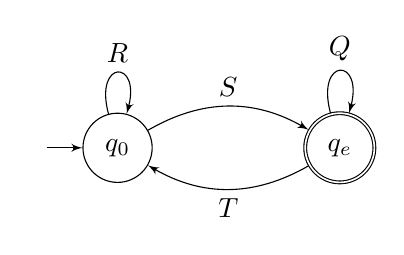
\begin{tikzpicture}[>=latex',/tikz/initial text=""]
	\node (q0) at (0bp,0bp)  [state, initial]   {$q_0$};
	\node (q1) at (80bp,0bp) [state, accepting] {$q_e$};

	\draw [loop above,->] (q0) to node[auto] {$R$} (q0);
	\draw [bend left,->]  (q0) to node[auto] {$S$} (q1);
	\draw [bend left,->]  (q1) to node[auto] {$T$} (q0);
	\draw [loop above,->] (q1) to node[auto] {$Q$} (q1);
\end{tikzpicture}
\\
ki jih prepišemo v en sam regularni izraz oblike:
\[ (R+SQ^*T)^*SQ^* \]

\begin{primeri}
\item Zapiši DKA za preverjanje deljivosti s 3 v binarnem sistemu? Zapiši še regularni izraz.\\
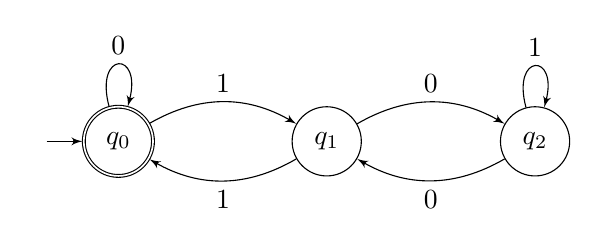
\begin{tikzpicture}[>=latex',/tikz/initial text=""]
	\node (q0) at (0bp,0bp)   [state, initial, accepting] {$q_0$};
	\node (q1) at (75bp,0bp)  [state]                     {$q_1$};
	\node (q2) at (150bp,0bp) [state]                     {$q_2$};

	\draw [loop above,->] (q0) to node[auto] {$0$} (q0);
	\draw [bend left,->]  (q0) to node[auto] {$1$} (q1);
	\draw [bend left,->]  (q1) to node[auto] {$1$} (q0);
	\draw [bend left,->]  (q1) to node[auto] {$0$} (q2);
	\draw [bend left,->]  (q2) to node[auto] {$0$} (q1);
 	\draw [loop above,->] (q2) to node[auto] {$1$} (q2);
\end{tikzpicture}
\ \\
Iz grafa eliminiramo eno stanje in zapišemo regularni izraz:
\[ (0+1(01^*0)^*1)^* \]
Možna pa je še ena rešitev, če eliminiramo drugo stanje.%napiši jo :P
\end{primeri}

\subsect{Desno-linearna gramatika $\rightarrow$ Nedeterministični končni avtomat z $\varepsilon$-prehodi}\label{DLG-eNKA}
Vhodno stanje avtomata je začetni simbol gramatike, nato pa stanja označujemo glede na končne in vmesne simbole, ki jih moramo še porabiti. Produkcije predstavljajo $\varepsilon$ prehode v avtomatu, preostali prehodi avtomata pa so črke, ki jih generiramo.

\Primer{Pretvori podano desno-linearno gramatiko v nedeterministični končni avtomat z $\varepsilon$-prehodi.
\begin{align*}
S &\rightarrow abA\ |\ aS\\
A &\rightarrow aa\ |\ bA\\
\end{align*}
\ \\[-25pt]%lol, hack
Po zgoraj opisanem postopku dobimo:\\ \ \\
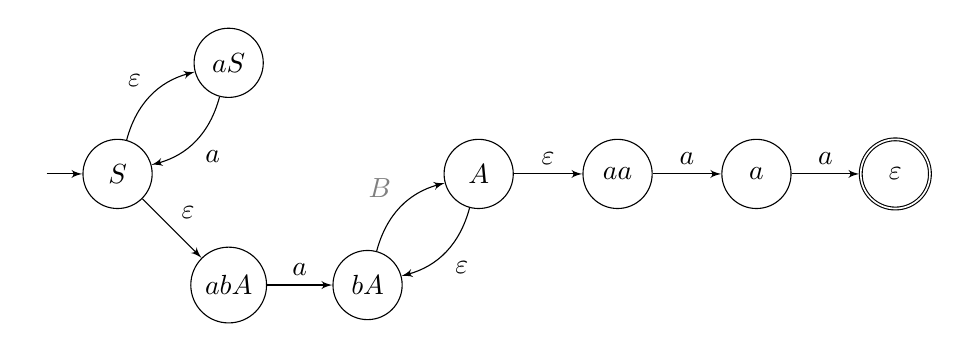
\begin{tikzpicture}[>=latex',/tikz/initial text=""]
	\node (S)   at (0bp,0bp)     [state, initial]  {$S$};
	\node (aS)  at (40bp,40bp)   [state]           {$aS$};
	\node (abA) at (40bp,-40bp)  [state]           {$abA$};
	\node (bA)  at (90bp,-40bp)  [state]           {$bA$};
	\node (A)   at (130bp,0bp)   [state]           {$A$};
	\node (aa)  at (180bp,0bp)   [state]           {$aa$};
	\node (a)   at (230bp,0bp)   [state]           {$a$};
	\node (e)   at (280bp,0bp)   [state,accepting] {$\varepsilon$};

	\draw [bend left,->]  (S) to node[auto] {$\varepsilon$} (aS);
	\draw [bend left,->]  (aS) to node[auto] {$a$} (S);
	\draw [->]  (S) to node[auto] {$\varepsilon$} (abA);
	\draw [->]  (abA) to node[auto] {$a$} (bA);
	\draw [bend left,->]  (bA) to node[auto] {\color{gray}$B$} (A);
	\draw [->]  (A) to node[auto] {$\varepsilon$} (aa);
	\draw [->]  (aa) to node[auto] {$a$} (a);
	\draw [->]  (a) to node[auto] {$a$} (e);
	\draw [bend left,->]  (A) to node[auto] {$\varepsilon$} (bA);
\end{tikzpicture}
}

\sect{Dokazovanje regularnosti jezika}\label{sec:Dokazovanje RJ}
%Dostikrat hočemo sestaviti regularen izraz za določen jezik in niti ne vemo ali je regularen izraz sploh regularen ali ne. Za to imamo nekaj metod za dokazovanje regularnosti jezika.%?false... ne moreš sestavit regularnega izraza, ki ni regularen :)
Kadar ugotavljamo, ali je nek jezik regularen, to lahko naredimo na več načinov:
\begin{items}
\item Pokažemo da je regularen:
	\begin{items}
	\item Jezik skonstruiramo v enem izmed modelov, ki sprejemajo regularne jezike:
		\begin{items}
		\item \nameref{sec:KA}
		\item \nameref{sec:RI}
		\item \nameref{sec:LLGDLG}
		\end{items}
	\end{items}
\item Dokažemo da ni regularen:
	\begin{items}
	\item Z uporabo leme o napihovanju za regularne jezike
	\item Z uporabo izreka Myhill-Nerode
	\item Dokažemo, da jezik ne spada niti v nek širši razred jezikov (glej \ref{sec:Dokazovanje KNJ})
	\end{items}
\end{items}

%?mislim, da je to pokrito tuki pri lemi...
%Opozorilo: Če zapišemo regularni izraz za jezik, ali naredimo končni avtomat, moramo dobro preveriti da ne obstaja kakšen protiprimer. Torej beseda ki je v jeziku in jo končni avtomat ali regularni izraz ne sprejme, ali obratno.\\
%Če nam ne uspe dokaza (da je ali da ni regularni jezik) do konca speljati, to ne moremo vzeti kot dokaz da ravno nasprotno drži. Velja da v takem primeru še nič ne vemo o regularnosti jezika.

\subsect{Lema o napihovanju za regularne jezike}\label{sec:Lema za RJ}
Lemo o napihovanju za regularne jezike uporabljamo za dokazovanje, da nek jezik ne spada v razred regularnih jezikov. 
\Def{Za vsak regularni jezik obstaja neka konstanta $n$, taka, da lahko vsako besedo $w$ iz jezika, daljšo od $n$, razbijemo na tri dele:
	\[ w=u\ v\ z \]
	Pri čemer velja:
	\begin{items}
	\item $|uv| \leq n$
	\item $|v| > 0$
	\item $uv^iz \in L,\ \forall i \geq 0$ (napihovanje)
	\end{items}
}
Ker dokazujemo da jezik ni regularen, moramo torej najti neko besedo, za katero pri napihovanju ne ostanemo znotraj jezika. Če nam tega z izbrano besedo ne uspe dokazati, še nismo dokazali da je jezik regularen -- edini pravi dokaz tega je konstrukcija jezika v enem izmed modelov, ki opisujejo regularne jezike.
\begin{center}
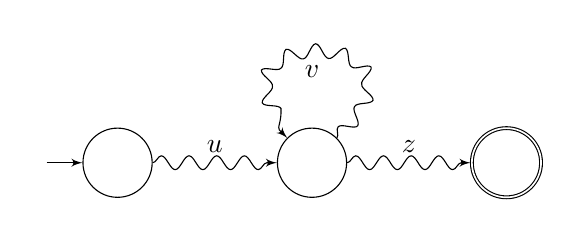
\begin{tikzpicture}[>=latex',/tikz/initial text=""]%scale=0.70, every state/.style={scale=0.70}]
	\node (q0) at (0bp,0bp)  [state, initial]   {};
	\node (q1) at (70bp,0bp) [state]            {};
	\node (q2) at (140bp,0bp) [state, accepting] {};

	\draw [decorate, decoration={snake},->]  (q0) to node[auto] {$u$} (q1);
	\draw [decorate, decoration={snake}, loop,->] (q1) to node[auto] {$v$} (q1);
	\draw [decorate, decoration={snake},->]  (q1) to node[auto] {$z$} (q2);
\end{tikzpicture}
\end{center}
Če zgornjo definicijo pogledamo v kontekstu končnih avtomatov, vidimo, da je $n$ gotovo večji od števila stanj, saj mora za napihovanje v avtomatu obstajati nek cikel, sicer bi bi veljalo $|v|=0$.

\subsect{Izrek Myhill-Nerode}


\subsect{Minimizacija končnih avtomatov}


\chap{Linearni jeziki}
%nismo delali pri TOR ;)
\sect{Linearne gramatike}\label{sec:LG}
\Def{Linearna gramatika je gramatika, ki ima na desni strani produkcij največ en vmesni simbol.\\
	Definirana kot četvorček $G=\langle N,T,P,S \rangle$, kjer so:
	\begin{items}
	\item N - množica spremenljivk oz. vmesnih simbolov
	\item T - množica znakov oz. končnih simbolov
	\item P - množica produkcij
	\item S - začetni simbol
	\end{items}
}
Posebna primera sta levo in desno-linearne gramatike, ki opisujeta regularne jezike (glej \ref{sec:LLGDLG})%?dvojina: amidoingitrite?
\begin{primeri}
\item Sestavi linearno gramatiko, ki sprejme jezik $L=\{ a^n b^n \ |\ n>0 \}$.
	\[ S \rightarrow aSb\ |\ ab \]
\item Sestavi linearno gramatiko, ki sprejme jezik $L=\{ 1 0^n 1 0^n 1\ |\ n \geq 2 \}$.
	\[ S \rightarrow 100A001 \]
	\[ A \rightarrow 0A0\ |\ 1 \]
\item Sestavi linearno gramatiko, ki sprejme jezik $L=\{ w w^R\ |\ w \in \{ 0,1 \} \}$.
	\[ S \rightarrow 1S1\ |\ 0S0\ |\ \varepsilon \]
\end{primeri}
\chap{Kontekstno-neodvisni jeziki}
\sect{Kontekstno-neodvisne gramatike}
%?oznake, izpeljave, ...
\Def{Kontekstno-neodvisna gramatika je definirana kot četvorček $G=\langle N,T,P,S \rangle$, kjer je:
\begin{items}
\item N - množica spremenljivk oz. vmesnih simbolov
\item T - množica znakov oz. končnih simbolov
\item P - množica produkcij
\item S - začetni simbol
\end{items}
}

%to je še treba nekam umestit
\Def{Kontekstno-neodvisna gramatika je dvoumna, kadar do nekega končnega niza lahko pridemo po več različnih izpeljavah.}

\Def{Kontekstno-neodvisna gramatika je deterministična, kadar za jezik, ki ga gramatika opisuje, obstaja vsaj ena gramatika, ki ni dvoumna. Ni nujno, da je taka gramatika, ki jo imamo - važno je, da taka gramatika obstaja.}

\subsect{Chomskyeva normalna oblika}
\Def{Kontekstno-neodvisna gramatika je v Chomskyevi normalni obliki, kadar nima nekoristnih simbolov, ter so vse produkcije naslednjih dveh oblik:\\
	\[ A \rightarrow a \]
	\[ A \rightarrow BC \]
	\[ a \in T,\ \ B,C \in N \]
}
\subsect{Greibachina normalna oblika}
\Def{Kontekstno-neodvisna gramatika je v Greibachini normalni obliki, kadar so vse produkcije oblike:\\
	\[ A \rightarrow a\gamma\]
	\[ a \in T,\ \ \gamma \in N^* \]
}

\sect{Skladovni avtomati}
\Def{Skladovni avtomat je definiran kot sedmerka $M=\langle Q, \Sigma, \Gamma, \delta, q_0, Z_0, F \rangle$, kjer je:
	\begin{items}
	\item $ Q $ - končna množica stanj
	\item $ \Sigma $ - vhodna abeceda
	\item $ \Gamma $ - skladovna abeceda
	\item $ \delta $ - funkcija prehodov, $\delta : Q \times (\Sigma \cup \{\varepsilon\}) \times \Gamma \rightarrow 2^{Q \times \Gamma^*}$%? zakaj U \varepsilon?
	\item $ q_0 $ - začetno stanje, $q_0 \in Q$
	\item $ Z_0 $ - začetni skladovni simbol, $Z_0 \in \Gamma$
	\item $ F $ - množica končnih stanj
	\end{items}
}
\subsect{Trenutni opis}
\Def{Trenutni opis je trojka $\langle q, w, \gamma \rangle \in Q \times \Sigma^* \times \Gamma^*$, pri čemer je $q$ trenutno stanje, $w$ preostanek vhodnega niza, ter $\gamma$ trenutna vsebina sklada}
\subsect{Relacija $\vdash$}
\Def{Relacija $\vdash$ nas pelje iz enega trenutnega opisa v drugega, če je ta prehod predviden v funkciji prehodov $\delta$:
	\[ \langle q, aw, Z\gamma \rangle \vdash \langle p, w, \gamma'\gamma \rangle \iff \langle p, \gamma' \rangle \in \delta(q,a,Z) \]
}
Uporabljamo tudi posplošeno relacijo $\vdash^*$, ki je ubistvu samo ena ali več-kratna uporaba relacije $\vdash$. Pove nam to, da pridemo iz enega trenutnega opisa do drugega, prek enega ali večih prehodov, pod pogojem, da vse vmesne prehode predvideva funkcija prehodov $\delta$.

\subsect{Jezik skladovnega avtomata}

\sect{Dokazovanje kontekstne-neodvisnosti jezika}\label{sec:Dokazovanje KNJ}
\subsect{Lema o napihovanju za kontekstno-neodvisne jezike}
\subsect{Ogdenova lema za kontekstno-neodvisne jezike}

\chap{Kontekstno-odvisni jeziki}
\sect{Kontekstno-odvisne gramatike}
\Def{Kontekstno-odvisna gramatika je definirana kot četvorček $G=\langle N,T,P,S \rangle$, kjer so:
	\begin{items}
	\item N - množica spremenljivk oz. vmesnih simbolov
	\item T - množica znakov oz. končnih simbolov
	\item P - množica produkcij
	\item S - začetni simbol
	\end{items}
	Pri tem je:
	\[ P \subset \left[\alpha_1 A \alpha_2 \rightarrow \alpha_1 \gamma \alpha_2 \right] \]
	\[ A \in N,\ \ \alpha_1,\alpha_2 \in (N \cup T)^*,\ \ \gamma \in (N \cup T)^+ \]
	Torej, niz z vsaj enim vmesnim simbolom preslikamo v nek drug niz. Pri tem je omejitev, da končnih simbolov ne smemo spreminjati.
}

\begin{primeri}
\item Sestavi kontekstno-odvisno gramatiko, ki sprejme jezik $L=\{ a^n b^n c^n\ |\ n>0 \}$.
	\begin{align*}
	S &\rightarrow aSBC\\
	S &\rightarrow aBC \\
	CB &\rightarrow HB \\
	HB &\rightarrow HC \\
	HC &\rightarrow BC \\
	aB &\rightarrow ab \\
	bB &\rightarrow bb \\
	bC &\rightarrow bc \\
	cC &\rightarrow cc \\
	\end{align*}
	S kompleksnejšo kontekstno-odvisno gramatiko sprejmemo tudi jezik $\{ a^n b^n c^n d^n\ |\ n>0 \}$
\end{primeri}
\subsect{Kurodova normalna oblika}
\Def{Kontekstno-odvisna gramatika je v Kurodovi normalni obliki, kadar so vse produkcije oblike:		\begin{align*}
	AB &\rightarrow CD\\
	A &\rightarrow BC \\
	A &\rightarrow B \\
	A &\rightarrow a \\
	\end{align*}
	\[ a \in T,\ \ A,B,C,D \in N \]
}

%--------------------------------TOR2 line--------------------------------------

\chap{Turingovi jeziki}
\sect{Zgodovina}
%I've got 23 problems, but a bitch ain't one. -Hilbert, 1900
%\br
Leta 1900 je Nemški matematik David Hilbert objavil seznam triidvajsetih nerešenih problemov v matematiki. Eden izmed Hilbertovih problemov (deseti po vrsti), je vprašanje, ali obstaja postopek, po katerem ugotovimo rešljivost poljubne Diofantske enačbe -- torej, ali lahko ugotovimo, če ima polinom s celoštevilskimi koeficienti $P(x_1, x_2, \dots, x_n)=0$, celoštevilsko rešitev.
%?več zgodovine tu :)
Kljub temu, da je Emil Post že leta 1944 slutil, da je problem nerešljiv, je to dokončno dokazal rus Jurij Matijaševič šele leta 1970 v svojem doktorskem delu. Med reševanjem problema pa so se matematiki že prej začeli ukvarjati s formalizacijo pojma postopka oz. algoritma. Intuitivna definicija tega se glasi nekako tako:
\Def{Algoritem je zaporedje ukazov, s katerimi se v končnem številu korakov opravi neka naloga.}
Pri tem pa ostaja še kar nekaj odprtih vprašanj, npr.:
\begin{items}
\item Kakšni naj bodo ukazi? 
	\begin{items}
	\item Osnovni - algoritem ima veliko korakov
	\item Kompleksni - prezapleteni ukazi so že sami algoritmi
	\end{items}
\item Koliko ukazov naj bo?
	\begin{items}
	\item Končno - ali je s končno množico res mogoče rešiti vsako nalogo?
	\item Neskončno - kakšen izvajalec ukazov je sposoben izvršiti neskončno različnih ukazov?
	\end{items}
\item So ukazi zvezni ali diskretni?
\item V kakšnem pomnilniku so ukazi shranjeni?
	\begin{items}%?verjetno ista vprašanja kot pri št. ukazov?
	\item Končnem - ali s končnim zaporedjem ukazov res lahko mogoče rešimo vsako nalogo?
	\item Neskončnem - \fixme%?
	\end{items}
\end{items}
Nekateri zgodnji poskusi formalizacije pojma algoritma so:%? zgodovinsko zaporedje, letnice, imena modelov, moar info
\begin{items}
    \item Rekurzivne funkcije (Kurt Gödel, Stephen Kleene) 
    \item Splošne rekurzivne funkcije (Jacques Herbrand, Kurt Gödel)
    \item Algoritmi Markova (Andrey Markov, ml.), %sin Markova http://en.wikipedia.org/wiki/Andrey_Markov_(Soviet_mathematician)
    \item Produkcijski sistem (Emil Post), %? je to http://en.wikipedia.org/wiki/Tag_system? 1943?
    \item Lambda račun (Alonso Church, 1936)
    \item Turingov stroj (Alan Turing, 1936)
\end{items}

\pagebreak
\sect{Turingovi stroji}
Turingov stroj se je uveljavil kot uporaben in preprost model računanja, ki zna izračunati vse kar se izračunati da (pod pogojem, da Church-Turingova teza drži). Alan Turing je svoj stroj izpeljal iz razmišljanja o tem, kako človek rešuje miselne probleme na papir. Pri tem je izbral tri sestavne dele:
\begin{items}
\item Nadzorno enoto (glava)
\item Čitalno okno (roka in vid)
\item Trak (papir)
\end{items}
V postopku formalizacije, pa je zaradi večje preprostosti, zahteval še, da je stroj sestavljen iz končno mnogo elementov, ter da deluje v diskretnih korakih.%?končno mnogo elementov? na kaj to cilja?
\ \\
\begin{center}
\begin{tikzturing}
	\node [on chain=trak] {Trak};
	\foreach \x in {1,2,...,5} {
		\node [cell] {$A_{\x}$};
	}
	\node      [cell]           {\ ...\ \ };
	\node (Ai) [cell, selected] {$A_i$};
	\node      [cell]           {\ ...\ \ };
	\node      [cell]           {$A_n$};
	\node      [cell]           {\color{gray}$B$};
	\node      [cell]           {\color{gray}$B$};
	\node      [cell]           {\ ...\ \ };
	\node      [cell, end]      {};

	%?must be a better way, zadnja črta niti ni naravnost
	\node (ne) at (110bp, 70bp) [head, minimum height=1.4cm, minimum width=3cm]  {Nadzorna enota};
	\draw (ne.south) -- (110bp, 25bp) -- (137.5bp, 25bp) [->] to (Ai.north);
	\node [below] at (Ai.south) {Čitalno okno};
\end{tikzturing}
\end{center}

\Def{Turingov stroj je definiran kot sedmerka $M=\langle Q, \Sigma, \Gamma, \delta, q_0, B, F \rangle $, kjer je:
\begin{items}
	\item $Q$ končna množica stanj
	\item $\Sigma$ končna množica vhodnih simbolov, $Q \cap \Sigma = \emptyset$
	\item $\Gamma$ končna množica tračnih simbolov, $\Sigma \subset \Gamma$
	\item $\delta$ funkcija prehodov: $Q \times \Gamma \rightarrow Q \times \Gamma \times \{L,D\}$,\\ kjer $L$ in $D$ označujeta premik levo ali desno
	\item $q_0$ začetno stanje, $q_0 \in Q$
	\item $B$ prazen simbol, $B \in \Gamma$
	\item $F$ množica končnih stanj, $F \subseteq Q$ 
\end{items}}
Stroj deluje tako, da v vsakem koraku opravi naslednje:
\begin{items}
	\item preide v neko stanje
	\item zapiše nov simbol v celico, ki je pod oknom
	\item okno premakne eno celico levo ali desno
\end{items}

\subsect{Trenutni opis}
\Def{$TO = \Gamma^* \times Q \times \Gamma^*$ je množica vseh trenutnih opisov.\\
Nek trenutni opis $\langle \alpha_1, q, \alpha_2 \rangle$, ali krajše $\alpha_1\ q\ \alpha_2$ opisuje konfiguracijo Turingovega stroja.
\br
\begin{center}
\begin{tikzturing}
	\node      [cell, minimum width=3.6cm] {$\alpha_1$};
	\node (Ai) [cell, selected]            {};
	\node      [cell, minimum width=3cm]   {$\alpha_2$\ \ \ };
	\node      [cell]                      {\color{gray}$B$};
	\node      [cell]                      {\color{gray}$B$};
	\node      [cell]                      {\ ...\ \ };
	\node      [cell, end]                 {};

	%?must be a better way, zadnja črta niti ni naravnost
	\node (ne) at (40bp, 60bp) [head]  {$q$};
	\draw (ne.south) -- (40bp, 25bp) -- (60.5bp, 25bp) [->] to (Ai.north);
	%\node [below, minimum width=4cm] at (alpha1.south) {$\alpha_1$};
	%\node [below, minimum width=4cm] at (alpha2.south) {$\alpha_2$\ \ \ \ };
\end{tikzturing}
\end{center}
\br
Čitalno okno je nad prvim znakom niza $\alpha_2$, iz tega lahko razberemo:
\begin{items}
	\item če je $\alpha_1 = \varepsilon$, je okno skrajno levo
	\item če je $\alpha_2 = \varepsilon$, je okno nad $B$ in so naprej sami $B$-ji
\end{items}}

\subsect{Relacija $\vdash$}
\Def{Če sta $u,v$ trenutna opisa iz množice $TO$, ter $v$ neposredno sledi iz $u$ v enem koraku Turingovega stroja, tedaj pišemo $u \vdash v$.
\br
Naj bo $x_1 \dots x_{i-1}\ q\ x_i \dots x_n$ trenutni opis:
\begin{items}
\item če je $\delta(q,x_i) = \langle p,Y,D \rangle$:\\
$x_1 \dots x_{i-1}\ q\ x_i \dots x_n \vdash x_1 \dots x_{i-1}\ Y\ p\ x_{i+1} \dots x_n$
\item če je $\delta(q,x_i) = \langle p,Y,L \rangle$: 
	\begin{items}
	\item če je okno na robu ($i=1$), se Turingov stroj ustavi, ker je trak na levi omejen.
	\item če okno ni na robu ($i>1$), potem: $x_1 \dots x_{i-2} x_{i-1}\ q\ x_i \dots x_n \vdash x_1 \dots\ x_{i-2} p\ x_{i-1}\ Y\ x_{i+1} \dots x_n$
	\end{items}
\end{items}}
Imamo pa tudi posplošeno relacijo $u \vdash^* v$, ki pove, da trenutni opis $v$ sledi iz $u$ v enem ali večih korakih.
\Def{$u \vdash^* v$, če obstaja tako zaporedje $x_i, (i \in [0, 1, \dots, k], k \geq 0)$, da velja $u=x_0, v=x_k$ in $x_0 \vdash x_1 \wedge x_1 \vdash x_2 \wedge \dots \wedge x_{k-1} \vdash x_k$
\br
Torej, trenutni opis $v$ sledi iz $u$, v $k$ korakih Turingovega stroja.}
\sect{Jezik Turingovega stroja}
\Def{Jezik Turingovega stroja je:
\begin{equation*}
L(M) = \{ w\ |\ w \in \Sigma^* \wedge \varepsilon\ q_0\ w \vdash^*\alpha_1\ q_F\ \alpha_2 \wedge \alpha_1,\alpha_2 \in \Gamma^*, q_F \in F \}
\end{equation*}
}
Z besedami to pomeni, da je jezik Turingovega stroja množica besed, ki če jih damo na vhod stroja, povzročijo, da se ta v končno mnogo korakih znajde v končnem stanju.
\ \\
\begin{center}
\begin{tikzturing}
	\node (Ai) [cell, selected]          {};
	\node      [cell, minimum width=4cm] {$w$\ \ \ \ \ };
	\node      [cell]                    {\color{gray}$B$};
	\node      [cell]                    {\color{gray}$B$};
	\node      [cell]                    {\ ...\ \ };
	\node      [cell, end]               {};

	%?must be a better way, zadnja črta niti ni naravnost
	\node (ne) at (90bp, 60bp) [head] {$q_0$};
	\draw (ne.south) -- (90bp, 25bp) -- (0bp, 25bp) [->] to (Ai.north);
\end{tikzturing}
\br
Začetna konfiguracija Turingovega stroja.
\end{center}
\Def{Jezik $L$ je Turingov jezik, če obstaja Turingov stroj $M$, tak, da je $L = L(M)$.}
\subsect{Ugotavljanje pripadnosti besed Turingovemu jeziku}
Pri vprašanju ali je neka beseda v jeziku, Turingove jezike ločimo na:
\begin{items}
\item Odločljive - obstaja algoritem, s katerim se lahko za poljubno besedo odločimo, ali pripada jeziku.
\item Neodločljive - v splošnem ni algoritma, ki bi za poljubno vhodno besedo z DA ali NE odgovoril na vprašanje pripadnosti.
	\begin{items}
	\item če je odgovor DA, to ugotovimo v nekem končnem številu korakov.
	\item če je odgovor NE, pa ni nujno, da se bo stroj kdaj ustavil.
	\end{items}
\end{items}

%?\fixme - vennov diagram beseda w znotraj L kroga... pomojm ne rabmo :P

%?where does this go?
%Terminologija: re (recursively enumerable, Turing recognizable)%?semi-decidable? 
%Rekurzivni jezik (decidable)%?where does this go?

\fixme - vennov diagram odločljivi jeziki znotraj Turingovih?

\Primer{Zapiši Turingov stroj, ki sprejema jezik $L=\{0^n 1^n | n \geq 1\}$\\
	Skica izvajanja stroja:
	\begin{items}
	\item $0^{n}1^{n}$ - vhodna beseda
	\item $X0^{n-1}1^{n}$ - zamenjamo najbolj levo $0$ z $X$
	\item $X0^{n-1}Y1^{n-1}$ - premaknemo okno desno do najbolj leve $1$ in jo zamenjamo z $Y$
	\item $XX0^{n-2}Y1^{n-1}$\\ 
		$XX0^{n-2}YY1^{n-2}$ - ponovimo in vidimo, da bomo niz sprejeli, če je prave oblike.
	\end{items}
	Turingov stroj zapišemo kot $M=\langle Q,\Sigma,\Gamma,\delta,q_0,B,F \rangle$:
	\begin{items}
    \item $Q=\{ q_0,q_1,q_2,q_3,q_4 \}$
    \item $\Sigma = \{ 0,1 \}$
    \item $\Gamma = \{ 0,1,B,X,Y \}$
    \item $F = \{ q_4 \}$
    \item $\delta$ bomo definirali s tabelo
	\end{items}

    Pomen stanj:
    \begin{items}
    \item $q_0$ - začetno stanje in stanje pred zamenjavo 0 z X
    \item $q_1$ - premikanje desno do 1
    \item $q_2$ - zamenjava 1 z Y in premikanje levo do X
    \item $q_3$ - najde X in se premik desno
    \item $q_4$ - končno stanje
    \end{items}

    Tabela prehajanja stanj:\\
	\begin{center}
    \begin{tabular}{ c | c c c c c}
	& 0 & 1 & B & X & Y\\ \hline
	$x_0$& $\langle q_1,X,D\rangle$ & -- & -- & $\langle q_3,Y,D\rangle$ & --\\
	$x_1$& $\langle q_1,0,D\rangle$ & $\langle q_2,Y,L\rangle$ & -- & $\langle q_1,Y,D\rangle$ & --\\
	$x_2$& $\langle q_2,0,D\rangle$ & -- & $\langle q_0,X,D\rangle$ & $\langle q_2,Y,L\rangle$ & --\\
	$x_3$& -- & -- & -- & $\langle q_3,Y,D\rangle$ & $\langle q_4,B,D\rangle$\\
	$x_4$& -- & -- & -- & -- & --\\
	\end{tabular}
	\end{center}
	\br
	Izvajanje stroja s trenutnimi opisi:
	\[ q_0 0011 \vdash X q_1 011 \vdash X 0 q_1 11 \vdash X q_2 0 Y 1 \vdash \dots \]
}
%?zapiski 2007 imajo tu še nekaj o turingovih jezikih
\subsect{Turingov stroj kot računalnik funkcij}
Imamo Turingov stroj, ki ima na traku neko število ničel, ki predstavljajo pozitivna naravna števila, ločena z enicami:
%	\[ 0^{i_1} 1 0^{i_2} 1  \dots 1 0^{i_k} \]
%?skupine ničel so i_1, i_2, ..., kjer so i naravna števila (mjbi i+1 ničel)  
\ \\
\begin{center}
\begin{tikzturing}
	\node (Ai) [cell, selected]            {};
	\node      [cell, minimum width=2cm]   {$0^{i_1}$\ \ \ };
	\node      [cell]                      {$1$};
	\node      [cell, minimum width=1.4cm] {$0^{i_2}$};
	\node      [cell]                      {$1$};
	\node      [cell]                      {\ ...\ \ };
	\node      [cell]                      {$1$};
	\node      [cell, minimum width=2.6cm] {$0^{i_k}$\ \ \ \ };
	\node      [cell]                      {\color{gray}$B$};
	\node      [cell]                      {\color{gray}$B$};
	\node      [cell]                      {\ ...\ \ };
	\node      [cell, end]                 {};

	%?must be a better way, zadnja črta niti ni naravnost
	\node (ne) at (70bp, 60bp) [draw, minimum width=2cm, minimum height=1.2cm]  {$q_0$};
	\draw (ne.south) -- (70bp, 25bp) -- (0bp, 25bp) [->] to (Ai.north);
\end{tikzturing}
\end{center}
Recimo, da se stroj po nekem številu korakov ustavi in ima na traku skupino ničel $0^m$, na levi in desni strani skupine pa same $B$-je. S tem je stroj morda izračunal neko funkcijo:
	\[ f^{(k)}:\mathbb{N}_+^k \rightarrow \mathbb{N}_+ \mbox{\ \ oz. \ \ } f(i_1, i_2, \dots, i_k) = m \]
%?\fixme - slika TS s skupino ničel na traku\br... pomojm ne rabmo :P
Funkcija $f$ ni nujno definirana za vsako $k$-terico iz $\mathbb{N}_+^k$, torej je parcialna funkcija, kadar pa je definirana povsod, pravimo da je totalna. Stroj se pri nedefiniranih $k$-tericah pač na neki točki ustavi in pri tem na traku ne pusti le ene skupine ničel, ali pa se sploh ne ustavi.
Isti turingov stroj hkrati računa več funkcij: $f^{(1)}, f^{(2)}, \dots f^{(k)}$.%?računa ali "lahko računa".. ne štekam ubistvu čist

\subsubsection{Parcialna rekurzivna funkcija}
\Def{Vsaka funkcija $f^{(k)}:\mathbb{N}_+^k \rightarrow \mathbb{N}$, ki jo lahko izračuna nek Turingov stroj, je parcialna rekurzivna funkcija. Če je $f^{(k)}$ definirana za vse $k$-terice, jo imenujemo totalna rekurzivna funkcija (včasih samo rekurzivna funkcija)}
Vse običajne aritmetične funkcije so parcialne ali celo totalne rekurzivne funkcije. V primerih si bomo pogledali nekaj primerov, tu pa jih nekaj naštejmo: $m+n,\ m*n,\ n!,\ 2^n,\ \lceil \log(n) \rceil,\ m^n,\ \dots$.
%so najdl primer, ki ne spada sem z diagonalizacijo
%na začetku so gledali totalne... pa so vidl da morajo parcialne
\begin{primeri}
\item
    Ali je $f(m,n)=m+n$ (parcialno) rekurzivna?\\
    Skica stroja, ki računa $m+n$:
    \begin{items}
    \item $0^m 1 0^m$ - vhodna beseda
    \item $B0^{m-1} 1 0^m$ - izbriši prvo ničlo
    \item $B0^{m+n}$ - premakni se do 1 in jo zamenjaj z 0
    \end{items}%?DN naredi cel stroj
\item
    Ali je $f(m,n)=m*n$ (parcialno) rekurzivna?\\
    Skica stroja, ki računa $m*n$:
    \begin{items}
    \item $0^m 1 0^n$ - vhodna beseda
    \item $0^m 1 0^n 1$ - premakni se na konec in zapiši 1 (ločnica za rezultat)
    \item $B 0^{m-1} 1 0^n 1$ - premakni se na začetek in izbriši 0
    \item $B 0^{m-1} 1 0^m 1 0^n$ - prekopiraj $n$ ničel za ločnico (in ničle)
    \item $B^{m} 1 0^m 1 0^{m*n}$ - ponavljaj tadva koraka, dokler ni več ničel pred prvo 1
    \item $B^{m+n+2}0^{m*n}$ - izbriši del, ki ne spada v rezultat 
    \end{items}%?naredi cel stroj
\end{primeri}

\sect{Razširitve in alternative Turingovemu stroju}
V tem odseku bomo spoznali nekaj razširitev Turingovega stroja in pokazali da so enako močne kot osnovni model. Poleg tega bomo naredili še pregled alternativnih modelov, za katere se je tudi izkazalo, da so enako močni.%, nato pa si bomo ogledali še nekaj stvari, ki jih Turingov stroj kljub vsemu ne more izračunati.

\Odmakni{Postopek dokazovanja}{Recimo, da je $\mathcal{M}$ razred modelov, za katerega želimo dokazati, da je ekvivalenten razredu Turingovih strojev. Poiskati moramo sistematičen, končen postopek S, ki poljubnemu stroju $M \in \mathcal{M}$ priredi nek Turingov stroj $M'$, ki je sposoben simulirati $M$.
\begin{center}
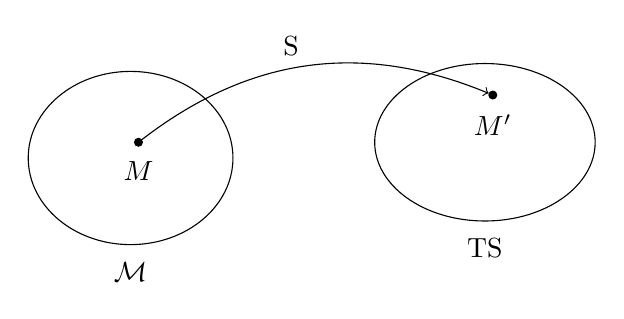
\begin{tikzpicture}[vert/.style={circle, draw,fill=black, inner sep=1pt}]
	\node (l) [vert] at (0.1cm, 0.2cm) {};
	\node [below=2pt] at (l.south) {$M$};
	\node (r) [vert] at (4.6cm, 0.8cm) {};
	\node [below=2pt] at (r.south){$M'$};

	\draw (0cm,0cm) ellipse (1.3cm and 1.1cm) node(le) {};
	\node at (le) [below=1.2cm] {$\mathcal{M}$};
	\draw (4.5cm,0.2cm) ellipse (1.4cm and 1.0cm) node(re) {};
	\node at (re) [below=1.1cm] {TS};

	\draw [bend left, ->] (l) to node[auto] {S} (r);
\end{tikzpicture}
\end{center}}
\subsect{Nadzorna enota kot pomnilnik}
Vsako stanje stroja, je sestavljeno iz dveh delov -- stanja avtomata, ter shrambe za tračne znake. Novo množico stanj zapišemo kot $Q=K\times\Gamma$, kjer je $K$ stara množica stanj in $\Gamma$ tračna abeceda.
\Primer{Sestavi Turingov stroj za razpoznavanje besed, pri katerih se prvi znak ne ponovi:\\
	Stroj $M=\langle Q,\Sigma,\Gamma,\delta,q_0,B,F \rangle$ zapišemo kot:
	\begin{items}
	\item $M=\langle Q, \{0,1\}, \{0,1,B\}, \delta, \langle q_0, B \rangle, B, F \rangle$
	\item $Q=\{ q_0, q_1 \} \times \{0,1,B\} = \{ \langle q_0, 0\rangle , \langle q_0, 1\rangle , \langle q_0, B\rangle , \langle q_1, 0\rangle , \langle q_1, 1\rangle , \langle q_1, B\rangle\} $
	\item $F=\{ \langle q_1, B \rangle \}$
	\item $\delta$ zapišemo kot:
		\begin{items}
		\item Shrani prvi znak besede v stanje stroja:\\
			$\delta(\langle q_0, B\rangle, 0) = \langle\langle q_1, 0 \rangle, 0, D\rangle$\\
			$\delta(\langle q_0, B\rangle, 1) = \langle\langle q_1, 1 \rangle, 1, D\rangle$
		\item Premakni okno v desno do prvega znaka, enakega shranjenemu:\\
			$\delta(\langle q_1, 0\rangle, 1) = \langle\langle q_1, 0 \rangle, 1, D\rangle$\\
			$\delta(\langle q_1, 1\rangle, 0) = \langle\langle q_1, 1 \rangle, 0, D\rangle$
		\item Če prebereš $B$, pojdi v končno stanje:\\
			$\delta(\langle q_1, 0\rangle, B) = \langle\langle q_1, B \rangle, karkoli \rangle$\\
			$\delta(\langle q_1, 1\rangle, B) = \langle\langle q_1, B \rangle, karkoli \rangle$
		\item Sicer se ustavi. To dosežemo tako, da ne definiramo prehodov:\\
			$\delta(\langle q_1, 0\rangle, 0)$ in $\delta(\langle q_1, 1\rangle, 1)$
		\end{items}
	\end{items}
}
\subsect{Večsledni trak}
Na traku imamo več kot eno sled, kar pomeni, da s traku beremo $k$-terice tračnih znakov, kar zapišemo kot: $\Gamma=\Gamma_1\times\Gamma_2\times\dots\times\Gamma_k$.
\ \\
\begin{center}
\begin{tikzturing}
	\node (Ai) [cell1, selected] {$A1_{0}$};
	\node at (0bp,-0.6cm) [cell2, selected] {$A2_{0}$};
	\node at (0bp,-1.2cm) [cell3, selected] {$A3_{0}$};

	\foreach \x in {1,2,3} {
		\node [cell1] {$A1_{\x}$};
		\node [cell2] {$A2_{\x}$};
		\node [cell3] {$A3_{\x}$};
	}

	\node [cell1] {\ ...\ \ };
	\node [cell2]  {\ ...\ \ };
	\node [cell3]  {\ ...\ \ };

	\node [cell1, end] {};
	\node [cell2, end] {};
	\node [cell3, end] {};

	%?must be a better way, zadnja črta niti ni naravnost
	\node (ne) at (40bp, 60bp) [draw, minimum width=2cm, minimum height=1.2cm]  {$q_0$};
	\draw (ne.south) -- (40bp, 25bp) -- (0bp, 25bp) [->] to (Ai.north);
\end{tikzturing}
\end{center}

\Primer{Sestavi Turingov stroj, ki preveri, ali je vhodno število praštevilo.\\
	Skica stroja:
	\begin{items}
	\item Trak ima tri sledi:
		\begin{items}
		\item na prvi sledi je vhodno število
		\item na drugi sledi je števec, ki na začetku hrani število 2
		\item tretjo sled uporabimo za delovno sled, na začetku je lahko prazna.
		\end{items}
	\item Stroj deluje tako:
		\begin{items}
		\item prepiši število s prve sledi na tretjo sled
		\item odštevaj število iz druge sledi od števila na tretji sledi
		\item če se odštevanje konča z 0, se ustavi (ni praštevilo)
		\item sicer število na drugi sledi povečaj za 1
		\item če je število na drugi sledi enako tistemu na prvi, sprejmemo (je praštevilo)
		\item sicer, ponovimo postopek
		\end{items}
	\end{items}
}
\subsect{Prestavljanje vsebine traku}
Recimo, da bi s traku radi vzeli nekaj zaporednih znakov tako, kot da bi jih izrezali iz traku in nato trak zlepili nazaj skupaj, izrezane simbole pa bi si pri tem seveda radi nekako zapomnili. Tudi to metodo realiziramo s pomočjo shrambe za tračne simbole v nadzorni enoti, a moramo pri tem paziti, da je funkcija prehodov pravilno napisana.
\br\fixme slika "gube" na traku in slika nadzorne enote
\Primer{Sestavi Turingov stroj, ki premakne vsebino traku za 2 celici v desno.\\
	Skica stroja:
	\begin{items}
    \item $Q$ vsebuje stanja oblike: $\langle q, A_1, A_2 \rangle;\ q \in \{ q_1, q_2 \},\ A_1, A_2 \in \Gamma$
    \item $\Gamma$ poleg ostalih znakov, vsebuje še poseben znak $X$, ki označuje izpraznjeno celico na traku
	\item $F=\{ q_2 \}$
	\item $\delta$ zapišemo kot:
		\begin{items}
		\item Prva koraka -- zapomni si in izprazni prvi in drugi znak:\\
			$\delta(\langle q_1, B, B\rangle, A_1) = \langle\langle q_1, B, A_1 \rangle, X, D \rangle $\\
			$\delta(\langle q_1, B, A_1\rangle, A_2) = \langle\langle q_1, A_1, A_2 \rangle, X, D \rangle $
		\item Zapomni si nov znak in prvega iz shrambe zapiši na trak:\\
			$\delta(\langle q_1, A_i, A_{i+1}\rangle, A_{i+2}) = \langle\langle q_1, A_{i+1}, A_{i+2} \rangle, A_i, D \rangle $
		\item Zadnja koraka -- zapiši vsebino shrambe na trak:\\
			$\delta(\langle q_1, A_{n-1}, A_{n}\rangle, B) = \langle\langle q_1, A_{n}, B \rangle, A_{n-1}, D \rangle $\\
			$\delta(\langle q_1, A_{n}, B\rangle, B) = \langle\langle q_2, B, B \rangle, A_{n}, L \rangle $
		\end{items}
	\end{items}
}

%?\fixme ... tu je razlagal tisto neizračunljivo funkcijo nad matrikami. btw, @zidar: poglej tor2-dodatno.pdf - tam govori o preroku

\subsect{Podprogrami}
\fixme
%?Imamo neka posebna stanja, ki signalizirajo vhod in izhod iz podprograma%?je tu govoril o dveh strojih?

\subsect{Turingov stroj z dvosmernim trakom}
Imamo Turingov stroj, ki ima trak neomejen v obe smeri. Vhodna beseda je na začetku napisana nekje na traku, okno pa je na prvem znaku besede.

%kako zbrišem črto pri prvem ...?
\begin{center}
\begin{tikzturing}
	\node      [cell]                    {\ ...\ \ };
	\node      [cell]                    {\color{gray}$B$};
	\node      [cell]                    {\color{gray}$B$};
	\node (Ai) [cell, selected]          {};
	\node      [cell, minimum width=4cm] {$w$\ \ \ \ \ };
	\node      [cell]                    {\color{gray}$B$};
	\node      [cell]                    {\color{gray}$B$};
	\node      [cell]                    {\ ...\ \ };
	\node      [cell, end]               {};

	%?must be a better way, zadnja črta niti ni naravnost
	\node (ne) at (95bp, 60bp) [draw, minimum width=2cm, minimum height=1.2cm]  {$q_0$};
	\draw (ne.south) -- (95bp, 25bp) -- (53.5bp, 25bp) [->] to (Ai.north);
\end{tikzturing}
\end{center}
\ \\
Stroj je definiran skoraj enako kot osnovni Turingov stroj, le funkcija prehodov $\delta$ je enostavnejša, saj ni treba skrbeti, kaj se zgodi, če zadanemo levi rob, kot pri običajnem Turingovemu stroju.
\br
\Trditev{Turingov stroj z dvosmernim trakom ni šibkejši od osnovnega Turingovega stroja.}
\Dokaz{Stroj se lahko vede kot da je omejen na levi. Na začetku izvajanja se premaknemo levo, zapišemo poseben znak, ki nam pomeni konec traku. Nato se premaknemo desno in stroj normalno izvajamo.}%to smo delali tudi na vajah - check it
\ \\
\Trditev{Turingov stroj z dvosmernim trakom ni močnejši od osnovnega.}
\Dokaz{Imamo Turingov stroj $M$ z dvosmernim trakom:
\ \\
%kako zbrišem črto pri prvem ...?
\begin{center}
\begin{tikzturing}
	\node [cell] {\ ...\ \ };

	\foreach \x in {-3,-2,-1} { \node [cell] {$A_{\x}$}; }
	\node (Ai) [cell, selected] {$A_{0}$};
	\foreach \x in {1,2,3} { \node [cell] {$A_{\x}$}; }

	\node [cell] {\ ...\ \ };
	\node [cell, end]      {};

	%?must be a better way, zadnja črta niti ni naravnost
	\node (ne) at (70bp, 60bp) [draw, minimum width=2cm, minimum height=1.2cm]  {$q_0$};
	\draw (ne.south) -- (70bp, 25bp) -- (95bp, 25bp) [->] to (Ai.north);
\end{tikzturing}
\end{center}
\ \\
Stroju $M$ priredimo dvosledni Turingov stroj $M'$. Zgornja sled nam bo predstavljala celice od $A_0$ naprej, spodnja pa vse tiste, levo od $A_0$:
\ \\
\begin{center}
\begin{tikzturing}
	\node (Ai) [cell1, selected] {$A_{0}$};
	\node at (0bp,-0.6cm) [cell2, selected] {\#};

	\foreach \x in {1,2,3} {
		\node [cell1] {$A_{\x}$};
		\node [cell2] {$A_{-\x}$};
	}

	\node [cell1] {\ ...\ \ };
	\node [cell2]  {\ ...\ \ };

	\node [cell1, end] {};
	\node [cell2, end] {};

	%?must be a better way, zadnja črta niti ni naravnost
	\node (ne) at (40bp, 60bp) [draw, minimum width=2cm, minimum height=1.2cm]  {$q_0$};
	\draw (ne.south) -- (40bp, 25bp) -- (0bp, 25bp) [->] to (Ai.north);
\end{tikzturing}
\end{center}

Stroj $M'$ deluje tako:
\begin{items}
\item naeenkrat dela le z eno sledjo
\item ko na drugi sledi vidi \#, zamenja aktivno sled
\item na zgornji sledi dela enako kot $M$
\item na spodnji se obrne smer premikanja
\end{items}
%(tu smo pomojem napisali še 2x isto)

%Formalizacija... ne bomo delal

%Sklep.. sta ekvivalentna - kar izračuna dvosmerni, lahko tudi osnovni.
%Izrek: Za jezik L obstaja TS z dvosmernim trakom, n.t.k., za L obstaja osnovni TS.

%nekdo je vprašal, če je bijekcija, pa je rekel, da ne čist?
}

\subsect{Večtračni Turingov stroj}
Večtračni Turingov stroj ima $k>1$ trakov, ki so neomejeni v obe strani. Poleg tega ima vsak trak svoje okno, ki se lahko neodvisno od ostalih premika ob vsakem koraku. Spet imamo na začetku vhodno besedo na prvem traku in je okno prvega traku na prvem znaku vhodne besede, na ostali trakovi pa so prazni.

\begin{center}
\begin{tikzturing}[cell11/.style={cell1,fill=white}, cell22/.style={cell2,fill=white}]
	\node [cell11] {\ ...\ \ };
	\node at (0bp,-1.5cm) [cell22]  {\ ...\ \ };
	\node at (0bp,-3.0cm) [cell3]  {\ ...\ \ };

	\node (Ai) [cell11, selected] {$w_{0}$};
	\node (Ai2) [cell22, selected] {\color{gray}$B$};
	\node (Ai3) [cell3, selected] {\color{gray}$B$};

	%?must be a better way, zadnja črta niti ni naravnost
	\node (ne) at (67bp, 60bp) [draw, minimum width=2cm, minimum height=1.2cm]  {$q_0$};
	\draw (ne.south) -- (67bp, 25bp) -- (29bp, 25bp) [->] to (Ai.north);
	\draw (ne.south) -- (67bp, -20bp) -- (29bp, -20bp) [->] to (Ai2.north);
	\draw (ne.south) -- (67bp, -65bp) -- (29bp, -65bp) [->] to (Ai3.north);

	\foreach \x in {1,2,3} {
		\node [cell11] {$w_{\x}$};
		\node [cell22] {\color{gray}$B$};
		\node [cell3] {\color{gray}$B$};
	}

	\node [cell11] {\ ...\ \ };
	\node [cell22]  {\ ...\ \ };
	\node [cell3]  {\ ...\ \ };

	\node [cell11, end] {};
	\node [cell22, end] {};
	\node [cell3, end] {};
\end{tikzturing}
\end{center}

\Def{Korak stroja $\delta$ opišemo kot:
	\[\delta = Q \times \Gamma^k \rightarrow Q\times(\Gamma\times\{ L,D,- \})^k \]
	Torej, na vsakem koraku dobimo iz trenutnega stanje, ter tračnega simbola vsakega traku, neko novo stanje, ter za vsak trak neodvisno nov simbol in premik.}

\Trditev{Večtračni Turingov stroj je enako močen kot osnovni model.}
\Dokaz{
	\Odmakni{($\Rightarrow$)}{Večtračni Turingov stroj uporabi le prvi trak.}
	\Odmakni{($\Leftarrow$)}{Turingovemu stroju $M$ s $k$-trakovi priredimo $2k$-sledni v obe strani neskončni Turingov stroj $M'$.
	Za vsak trak stroja $M$ imamo tako dve sledi v $M'$ -- na zgornji sledi je zapisana oznaka $X$, ki pove, kje naj bi bilo okno na tem traku stroja $M$, na spodnji sledi pa je zapisana vsebina tega traku stroja $M$.

\begin{center}
\begin{minipage}[t]{6cm}
\begin{tikzturing}[cell11/.style={cell1,fill=white}]
	\node [cell11] {\ ...\ \ };
	\node at (0bp,-1.5cm) [cell2]  {\ ...\ \ };

	\node (Ai) [cell11, selected] {$a$};

	\node       [cell2] {$c$};
	\node (Ai2) [cell2, selected] {$d$};

	%?must be a better way, zadnja črta niti ni naravnost
	\node (ne) at (50bp, 60bp) [draw, minimum width=2cm, minimum height=1.2cm]  {$q$};
	\draw (ne.south) -- (50bp, 25bp) -- (29bp, 25bp) [->] to (Ai.north);
	\draw (ne.south) -- (50bp, 25bp) -- (57bp, 25bp) [->] to (Ai2.north);

	\node [cell11] {\color{gray}$B$};

	\node [cell11] {\color{gray}$B$};
	\node [cell2]  {\color{gray}$B$};

	\node [cell11] {\ ...\ \ };
	\node [cell2]  {\ ...\ \ };

	\node [cell11, end] {};
	\node [cell2, end] {};
\end{tikzturing}
$k$-tračni stroj $M$
\end{minipage}
\begin{minipage}[t]{6cm}
\begin{tikzturing}
	\node [cell1] {\ ...\ \ };
	\node at (0bp,-0.6cm) [cell2]  {\ ...\ \ };
	\node at (0bp,-1.2cm) [cell3]  {\ ...\ \ };
	\node at (0bp,-1.8cm) [cell4]  {\ ...\ \ };

	\node [cell1] {$X$}; \node [cell1] {\color{gray}$B$};
	\node [cell2] {$a$}; \node [cell2] {\color{gray}$B$};
	\node [cell3] {\color{gray}$B$}; \node [cell3] {$X$};
	\node [cell4] {$c$}; \node [cell4] {$d$};

	\node (Ai) [cell1,selected] {\color{gray}$B$};
	\node      [cell2,selected] {\color{gray}$B$};
	\node      [cell3,selected] {\color{gray}$B$};
	\node      [cell4,selected] {\color{gray}$B$};

	\node [cell1] {\ ...\ \ };
	\node [cell2] {\ ...\ \ };
	\node [cell3] {\ ...\ \ };
	\node [cell4] {\ ...\ \ };

	\node [cell1, end] {};
	\node [cell2, end] {};
	\node [cell3, end] {};
	\node [cell4, end] {};

	%?must be a better way, zadnja črta niti ni naravnost
	\node (ne) at (60bp, 60bp) [draw, minimum width=2cm, minimum height=1.2cm]  {$q$};
	\draw (ne.south) -- (60bp, 25bp) -- (85.5bp, 25bp) [->] to (Ai.north);

\end{tikzturing}
$2k$-sledni stroj $M'$
\end{minipage}
\end{center}
\br

Stroj $M'$ torej hrani trenutni položaj na trakovih s dodatno sledjo, ki ima v ustrezni celici zapisan simbol $X$.
\br
Poleg tega pa pri $M'$ potrebujemo še drugačno nadzorno enoto, ki hrani:
\begin{items}
\item Stanje stroja
\item $k$ tračnih simbolov
\item Števec na intervalu $[0,k]$, ki nam pove, koliko simbolov $X$ je še desno od trenutnega položaja okna.
\end{items}
\ \\
Stroj $M'$ simulira en korak stroja $M$ tako da:
\begin{items}
\item Okno pomika v desno
\item Ko na neki sledi naleti na simbol $X$:
	\begin{items}
	\item V nadzorno enoto shrani simbol iz naslednje sledi
	\item Zmanjša števec za 1.
	\end{items}
\item Ko števec doseže 0, se začne pomikati v levo
\item Ko naleti na simbol $X$
	\begin{items}
	\item Zamenja tračni simbol na naslednji sledi, enako kot bi naredil stroj $M$
	\item Premakne se levo ali desno, enako kot bi naredil stroj $M$
	\item Poveča števec za 1
	\end{items}
\item Ko števec doseže $k$, nadzorna enota preide v novo stanje, enako kot bi naredil stroj $M$
\end{items}
\ \\
En korak stroja $M$ torej simuliramo s končno dolgim sprehodom v desno in levo.
}}%konec dokaza

\Neurejeno

\subsect{Nedeterministični Turingov stroj}
$\delta:Q\times\Gamma \rightarrow 2^{Q\times\Gamma\times\{ L,D,- \}}$
.. ... ... toda le končno mnogo

\Primer{
$\delta(0, a) = \{ \langle q_1, b, L \rangle, \langle q_2, c, D \rangle, \langle q_3, a, L \rangle, \langle q_2, B, L \rangle \}$
stroj bo izbral tisto preslikavo, ki ga vodi k sprejetju vhodne besede, če je to vodi.
...: ...
}

Nedeterministični Turingov stroj sprejme besedo, kadar obstaja končno zaporedje korakov, po katerem pridemo do končnega stanja.

\Trditev{Nedeterministični Turingov stroj zmore vse kar zmore osnovni Turingov stroj.}
\Dokaz{Funkcija prehodov $\delta$ osnovnega TS je le poseben primer funkcije $\delta$ nedeterminističnega Turingovega stroja.}
\Trditev{Nedeterministični Turingov stroj ni močnejši od osnovnega modela.}
\Dokaz{simulacija NTS z osnovnim:
%slika 
%
% d     a
%   |-------
% q |   o
%
%
naj ima njegov program delta v vsaki množici delta q a kvečjemu r možnih potez(oz. elementov delta? množice)
Stroju M priredimo trisledni osnovni TS M'
na prvi sledi ima M' vhodno besedo M
na drugi sledi M' generira/izpisuje navodila eno za drugim. navodila so besed nad {1,2...r} v leksikografskem redu.
npr r=3 ... 1,2,3, 11, 12, 13, 21, 22, 23, 31, 32, 33, 111, 112, 
na tretji sledi simulira stroj M, kot da bi M sam izbral svoje poteze, skladno s tekočim navodilom.% ajprov?

Natančneje:
M' na 2. sledi sestavi novo, naslednje navodilo
prepiše vhodno besedo s prvega na tretji sled (prej lahko tretha sked zbrupe(tretjo sled zbriše), če je kaj ostalo od prej)
na tretji sledi oponaa stroj M, kot da bi ta izbiral svoje poteze po tekočem navodilu.

pri tem: 
če M' pride do konca navodila, in je tedaj v končnem stanju, besedo sprejmemo.
sicer če ne pride do konca navodila, ali pa se ustavi v nekončnem stanju, potem pojdi v (natančneje prva vrstica)
%a to je tko k depth first? recimo no
%kaj če se navodilo zacikla? to se da rešit... i dunno :)
%aha, ne more se - ... ker ima končno mnogo nečesa
%hm a se lahko nts konča, simulator pa zacikla? nas ne briga.
}
%Trditev: če M sprejme besedo, jo sprejme tudi M' 
%Dokaz: 
%izrek: za L obstaja nts, ntk za L obstaja osnovni ts.

\subsect{Večdimenzionalni Turingov stroj}
... k>=2
premikamo se lahko v 2k smeri
...
...
...
\Primer{k=3\\
\fixme - 3D trak s trollhands puščico na celico
}

\subsubsect{Turingov stroj z več okni}
\fixme - slika z večimi okni

%-----------------------predavanja 4-------------------------------
%Turing se je zgledoval po človeku

%drugi po funkcijah
%kaj je računanje, izračunljivost, algoritem... na številsko-teoretskih funkcijah f:N->N ... totalne/parcialne
%študirali so totalne f:N->N
%Cilji: storga mat. definicija pojmov s tem da zadosti 2 stvarem:
	%zajeti mora vse "izračunljve funkcije" (vse kar si lahko zamislimo kot problem za računanje)
	%za vsako tako f, mora biti razviden mehaničen postopek za izračun njenih vrednosti
%(HK,HG,lambda)

%zgledovanje po (naravnem) jeziku
%Postov stroj, Algoritmi Markova
%računanje oz. reševanje mat. problemov je pri človeku preoblikovanje množice besed v drugo (opis problema, v opis rešitve)

\subsect{Rekurzivne funkcije}
%(GK) Gödel, Kleene
Definiral je funkcije: ničelna, naslednik, projekcija.
Dodal je pravili sestavljanja, kako iz začetnih in že sestavljenih dobimo novo: kompozicija, primitivna rekurzija. %grafek vseh sestavljivih (primitivno rekurzivnih) funkcij \_/
%godel je probal par funkcij in mu je ratal... kar je blo lepo... še lepš pa:
Konstrukcija take funkcije opisuje tudi mehanični postopek za izračun vrednosti funkcije, to pa je tudi kandidat za formalni opis pojma algoritma.
\br
Ampak... Ackermannova funkcija ni primitivno rekurzivna in narašča hitreje od vsake funkije, ki pripada primitivno rekuzivnim.
%\[ A(m,n) { n+1, m=0 
%          { A(m-1,1), m>0 in n=0
%          { A(m-1,1, A(m, n-1)), m>0 in n>0\]%obstaja šeena def

Kleene leta 1936 doda šeeno pravilo sestavljanja, $\mu$-operacija. %to zato, da naredi totalno, čeprov je možno parcialne
\Def{Totalne š.t. funkcije $f:N^k\leftarrow N$, ki se dajo konstruirati iz treh začetnih funkcij s končno mnogo uporabami treh pravil sestavljanja se imenujejo rekurzivne funkcije.}

Razred rekurzivnih funkcij
...
\begin{items}
\item $\zeta(n)=0 \forall n$ - ničelna
\item $\sigma(n)=n+1 \forall n$ - naslednik
\item $\pi(n_1, n_2, \dots, n_k)=n_i \forall n..$ - projekcija
\end{items}
Pravila sestavljanja
1. Če so dane funkcije $g:N^m \leftarrow N$ in $n_h:N^k \leftarrow N$, kjer i 1-m, potem je funkcija $f(n_1,n_2,\dots,n_k) \mbox{ po def } g(h_{1}(n_1,n_2,\dots,n_k),\dots,h_m(n_1,n_2,\dots,n_k))$ sestavljena s kompozicijo funkcij
2. Če sta dani funkciji $g:N^k \leftarrow N$ in $h:N^{k+1}  \leftarrow n$, potem je $f$ definiriana z:
	\[f(n_1, n_2, \dots, n_k, 0) \mbox{ po def } g(n_1, n_2, \dots, n_k)\]
	\[f(n_1, n_2, \dots, n_k, m+1) \mbox{ po def } h(n_1, n_2, \dots, n_k, m), f(n_1, n_2, \dots, n_k, m)), za m \geq 0\]
sestavljeno s .... in $g$ in $h$
3. Če je funkcija $g:N^{k+1} \leftarrow N$ taka, da za vsako $k$-terico naravnih števil $n_1, n_2, \dots, n_k$ obstaja n ..neki.. m, da je $g(n_1, n_2, \dots, n_k, m) = 0$, potem je funkcija:
\[ f(n_1, n_2, \dots, n_k) po def \mu x g(n_1, \dots, n_k, x)\]
sestavljena z $\mu$-operacijo iz funkcije $g$.
%Pri tem je $\mu$-operacija definirana z:
%\[ \mu x g(n_1, \dots, n_k, x) po def je najmanjši X, pri katerem je g (n_1, \dots n_k, X) = 0\]

%---
Konstrukcija rekurzivne funkcije $f$ je končno zaporedje $f_1,f_2,\dots,f_L$, kjer je $f_L=f$ in je vsaka funkcija $f_i$ vmes, bodisi začetna, bodisi sestavljena z enim izmed treh pravil iz predhodnic v tem zaporedju %glej grafek

%zaeenkrat nismo našli Ackermann2, ki bi to pokvarila :)
\Odmakni{Povzetek}{Algoritem po Gödel-Kleenu(GK) je ravno konstrkucija rekurzivne funkcije.\\
	Računanje po GK je izračun vrednosti funkcije tako, kot jo narekuje njena konstrukcija.\\
	Funkcija je izračunljiva po GK, če je rekurzivna.}

\subsubsect{Splošne rekurzivne funkcije}
Herbrand je študiral, kako poljubno ŠT funkcijo definirati s sistemom enačb.

f je neznana funkcija, $g_1, g_2, \dots g_m$ pa znane %mestnost?
f-je in g-je poljubno vstavljamo kot argumente v druge, nato pa nekatere dobljene izraze izenačimo, potem pa če ima dobljeni sistem natanko eno rešitev za funkcijo f, potem je f rekurzivna.%preden je umrl v alpah je poslal tako pismo gödlu.. katerega leta?
Gödel je dodal dve dodatni zahtevi... f se sme na levi strani enačb sme pojaviti v obliki $f(g(...), g_k(...)$ %Herbrand je dovoljeval f(g...f...g), kar je preveč divje
f naj bo povsod na $N^k$ definirana (totalna).
Če se jo da zapisati s takim sistemom, je zapisana s standardnim sistemom. Tedaj je tak sistem za f z oznako $\varepsilon(f)$.

Kakšna so pravila za računanje vrednosti $f(n_1, n_2, \dots, n_k)$ iz $\varepsilon(f)$. %leta 1934 je ugotovil, da
Pravili sta samo 2.
1. v enačbi lahko vse pokave iste spremenljivke zamenjamo z istim naravnim številom???
2. v enačbi lahko pojave funkcije zamenjamo z njeno vrednostjo

Godel trdi: funkcija f za katero obstaja $\varepsilon(f)$ , se imenjue splošno rekurzivna%it's first def'd here.

\Odmakni{Povzetek}{Algoritem po Herbrant-Gödlu(HG) je $\varepsilon(f)$.\\
	Računanje po HG je izračun vrednosti funkcije $f(n_1,\dots,n_k)$ iz $\varepsilon(f)$ z uporabo pravil 1,2.\\%izr. je, sta rekla... oz je samo Gödel reku... oh, snap :D
	Funkcija je izračunljiva po HG, če je splošno rekurzivna.}

\subsect{$\lambda$-račun}%1932,1933 Alonso Church
Imamo vhodni izraz, ki opisuje neko funkcijo f in argumente $n_1, \dots, n_k$.

Kako je funkcija opisana?
Začetni $\lambda$-term

Cilj: preoblikovati začetni $\lambda$-term v končni $\lambda$-term, tak, ki bo opisoval ravno vrednost $f(n_1, \dots, n_k)$
%this shit is exclusive :D

To preoblikovanje dosežemo z uporabo t.i. redukcij. Ta\\
bodisi preimenuje spremenljivko v $\lambda$-termu, $(\alpha)$
bodisi uporabi neko funkcijo nad njenimi argumenti.$(\beta)$ %a se da $\lambda$-term makro, ki bo pogledal nazaj in se pravilno sklonil? :D

$t0->t1->...->tK$
$f, n1, n2, ... nk$....$f(n_1, \dots, n_k)$

\Def{funkcija, ki jo je možno predstaviti in računati v tem lambda računu, taka funkcija je $\lambda$-definabilna}%fo'real!

\Odmakni{Povzetek}{Algoritem po Churchu je $\lambda$-term.\\
	Računanje po Churchu je preoblikovanje začetnega $\lambda$-terma v končni $\lambda$-term z redukcijami.\\
	Funkcija je izračunljiva po Churchu, če je $\lambda$-definabilna.}

%zgledovanje po jeziku (glej gor)

\subsect{Postov Stroj}%1936, Post
%podoben turingovemu
%nadzorna enota
%trak s celicami
%okno
%+vrsta z znaki povezana v nadz enoto in iz nadzorne grejo lahko na konec vrste

Model je podoben Turingovemu stroju, z naslenjimi spremembami:
\begin{items}
\item s traku le bere znake
\item Uporablja vrsto znakov
\end{items}

Korak: prebere iz celice pod oknom znak in iz začetka vrste znak. na podlagi teh dveh znakov in stanja bo premaknil okno, nov znak dal na konec vrste in prešel v novo stanje.

%iz jezika? how? najprej: graf: opis problema pride v začetno vozlišče, nato po grafu potuje in se spreminja, dokler ne pride v končno stanje - rezultat. besedi se odreže prvi znak in glede na to se izbere pot v grafu, ali spremeni besedo, etc.. stroj to simulira.
%zgleda končen... kaj zdj? trak je končen, vrsta, stanja, ... %i dunno lol

\Odmakni{Povzetek}{Algoritem po Postu je program Postovega stroja.\\
	Računanje po Postu je izvajanje programa Postovega stroja.\\
	Funkcija je izračunljiva po Postu, če njeno vrednost lahko izračuna Postov stroj.}

\subsect{Algoritmi Markova}%194..
Imamo abecedo $\Sigma$, končno zaporedje produkcij:
$x_1 \leftarrow y_1$
$x_2 \leftarrow y_2$
...
$x_n \leftarrow y_n$
$x,y \in \Sigma^*$%string v string

Produkija preoblikuje besedo tako da v tej besedi nadomesti skrajno levi pojav $x_i$ z $y_i$ %slikca beseda prej potem... x1->y1
%samo leva izpeljava, WTF?

Algoritem je zaporedje korakov, ki postopno preoblikuje začetno besedo v končno. V vsakem koraku se trenutna beseda preoblikuje s prvo (levo) možno produkcijo.

\Odmakni{Povzetek}{Algoritem po Markovu je gramatika.\\
	Računanje po Markovu je preoblikovanje vhodne besede z dano gramatiko.\\
	Funkcija je izračunljiva po Markovu, če njeno vrednost računa kaka gramatika}

%poudarki: kaj imajo skupnega?
%razumno zmogljivi - končo različnih ukazov, vsak ukaz se izvede v končno korakih / času, v enem koraku se opravi končno veliko dela, učinek ukaza je predvidljiv(tudi nedeterminističnem... mjbi kvantni ne).
%potencialno neskončen spomin brez omejitev dostopa

%zdj pa neki za lepe sanje:
%vsi so se matral še kj več narest
\sect{Church-Turingova teza}
Church je postavil domnevo... "algoritem" debela leftright puščica algoritem po Churchu %lol, kar sm js reku je algoritem :P glej sigma pri Churchu... Gödel ga je nekoliko zavrnil, vmes turing neodvisno do podobnega

Turing je postavil domnevo: "algoritem"  debela leftright puščica algoritem po Turingu

%Kdo je imel prav? oba, lol

%lol, trolla moje latex skille :)

Church-Turingova teza: algoritem intuitivno debela leftright puščica algoritem po Turingu%bolj točno program turing stroja in turing zato, ker je najbl cute
\end{document}